\documentclass{report}

\input{~/dev/latex/template/preamble.tex}
\input{~/dev/latex/template/macros.tex}

\title{\Huge{}}
\author{\huge{Nathan Warner}}
\date{\huge{}}
\pagestyle{fancy}
\fancyhf{}
\lhead{Warner \thepage}
\rhead{}
% \lhead{\leftmark}
\cfoot{\thepage}
%\setborder
% \usepackage[default]{sourcecodepro}
% \usepackage[T1]{fontenc}

\begin{document}
    % \maketitle
        \begin{titlepage}
       \begin{center}
           \vspace*{1cm}
    
           \textbf{C++} \\
           From control structures  \\ through objects
    
           \vspace{0.5cm}
            
                
           \vspace{1.5cm}
    
           \textbf{Nathan Warner}
    
           \vfill
                
                
           \vspace{0.8cm}
         
           
\includegraphics[width=0.4\textwidth]{~/niu/seal.png}
                
           Computer Science \\
           Northern Illinois University\\
           September 1, 2023 \\
           United States\\
           
                
       \end{center}
    \end{titlepage}
    \tableofcontents
    \pagebreak \bigbreak \noindent
    \begin{center}
        \begin{Huge}
           \textbf{Preface} 
        \end{Huge}
    \end{center}
    \bigbreak \noindent 
    \line(1,0){490}
    \bigbreak \noindent 
    \href{https://github.com/JiaRuiShao/CPP/blob/master/Starting%20Out%20with%20C%2B%2B%20from%20Control%20Structures%20to%20Objects%208%20Tony%20Gaddis.pdf}{(Textbook Access (pdf))}
    \bigbreak \noindent 
    This document serves as a supplementary guide to \textit{C++ from Control Structures Through Objects by Tony Gaddis}. While the original text is geared towards beginners, this guide aims to assist those who already have programming experience, possibly in other languages.
    \bigbreak \noindent 
    To streamline the content and focus on aspects that are unique or nuanced in C++, this guide omits Chapters I and II of the original text. Instead, you will find a concise overview of the following foundational topics:
    \begin{itemize}
        \item Language Features
        \item The complier
        \item Boilerplate Code Structure
        \item Commenting Practices
        \item Data Types, Modifiers, Qualifiers, and Inference
        \item Type introspection
        \item Operators and Special Symbols
        \item The Using Directive
        \item Scope 
        \item Preprocessor Directives
        \item Standard Input/Output Techniques
    \end{itemize}
    \bigbreak \noindent
    Please note that basic elements like variables and arithmetic operations are not covered in this guide, under the assumption that readers are already familiar with these core computing concepts.

    %
    % This document will contain information found in \textit{C++ from control structures through objects by Tony Gaddis}. Although, this document will \textbf{not} be catered towards a beginning programmer, it is designed for those who may have experience in other languages. For this reason, this document will be omitting chapters I and II. In their place, there will  be a brief rundown on topics such as:
    % \begin{itemize}
    %     \item Boilerplate program
    %     \item Comments
    %     \item Includes
    %     \item Data types and modifiers
    %     \item Determine size of data types
    %     \item Symbols
    %     \item Input/Output
    %     \item scope
    % \end{itemize}
    % \bigbreak \noindent 
    % As an additional note, there \textbf{will not} be a section regarding variables, assignment statements, and arithemetic operations, as these are trivial to anyone familiar with concepts of computing.
    
    \pagebreak \bigbreak \noindent 
    \vspace{2.2in} \\
    \begin{Huge}
        \textbf{C++ from control \\ structures through objects}
    \end{Huge}
    \bigbreak \noindent 
    \line(1,0){490}
    \bigbreak \noindent 
    \section{\LARGE The C++ Language}
    \bigbreak \noindent 
    C++ is a high-level, general-purpose programming language that was developed as an extension of the C programming language. Created by Bjarne Stroustrup, the first version was released in 1985. C++ is known for providing both high- and low-level programming capabilities. It is widely used for developing system software, application software, real-time systems, device drivers, embedded systems, high-performance servers, and client applications, among other things. C++ is praised for its performance and it's used for system/software development and in other fields, including real-time systems, robotics, and scientific computing.
    \bigbreak \noindent 
    \subsection{Key Features}
    \bigbreak \noindent 
    \begin{itemize}
        \item \textbf{Object-Oriented:} C++ supports Object-Oriented Programming (OOP), which allows for better organization and more reusable code. Concepts like inheritance, polymorphism, and encapsulation are available.
        \item \textbf{Procedural:} While C++ supports OOP, it also allows procedural programming, just like its predecessor C. This makes it easier to migrate code from C to C++.
        \item \textbf{Low-level Memory Access:} Like C, C++ allows for low-level memory access using pointers. This is crucial for system-level tasks.
        \item \textbf{STL (Standard Template Library):} C++ comes with a rich set of libraries that include pre-built functions and data types for a variety of common programming tasks, from handling strings to performing complex data manipulations.
        \item \textbf{Strongly Typed:} C++ has a strong type system to prevent unintended operations, although it does provide facilities to bypass this.
        \item \textbf{Performance:} One of the most significant advantages of C++ is its performance, which is close to the hardware level, making it suitable for high-performance applications.
        \item \textbf{Multiple Paradigms:} In addition to procedural and object-oriented programming, C++ also supports functional programming paradigms.
    \end{itemize}

    \pagebreak \bigbreak \noindent 
    \section{\LARGE The Compiler}
    \bigbreak \noindent 
    Unlike interpreted languages like Python or JS, C++ is a compiled language. The C++ compiler is a toolchain that takes C++ source code files and transforms them into executable files that a computer can run. The process involves several stages to get from human-readable C++ code to machine code that a CPU can execute.
    \bigbreak \noindent 
    Here's a general breakdown of the C++ compilation process:
    \bigbreak \noindent 
    \subsection{Preprocessing}
    \bigbreak \noindent 
    In this stage, the \textbf{preprocessor} takes care of directives like \#include, \#define, and \#ifdef. It replaces macros with their actual values and includes header files into the source code. The output of this stage is an expanded source code file.
    \begin{itemize}
        \item \textbf{Macro Replacement:} Replace macros with their respective values.
        \item \textbf{File Inclusion:} Include header files specified by \#include directives.
        \item \textbf{Conditional Compilation:} Code between \#ifdef and \#endif (or related preprocessor conditionals) is included or excluded based on the condition.
    \end{itemize}

    \bigbreak \noindent 
    \subsection{Lexical Analysis}
    \bigbreak \noindent 
    The expanded source code is then tokenized into a sequence of tokens (keywords, symbols, identifiers, etc.). This stage is known as lexical analysis or scanning. The lexer converts the character sequence of the program into a sequence of lexical tokens.

    \bigbreak \noindent 
    \subsection{Syntax Analysis}
    \bigbreak \noindent 
    The sequence of tokens is then parsed into a syntax tree based on the grammar rules of the C++ language. This stage is known as syntax analysis or parsing. The parser checks whether the code follows the syntax rules of C++ and constructs a syntax tree which is used in the subsequent stages of the compiler.

    \bigbreak \noindent 
    \subsection{Semantic Analysis}
    \bigbreak \noindent 
    Semantic rules like type-checking, scope resolution, and other language-specific constraints are verified at this stage. For example, it ensures that variables are declared before use, that functions are called with the correct number and types of arguments, etc.

    \bigbreak \noindent 
    \subsection{Intermediate Code Generation}
    \bigbreak \noindent 
    The syntax tree or another intermediate form is then converted into an intermediate representation (IR) of the code. This is often a lower-level form of the code that is easier to optimize.

    \bigbreak \noindent 
    \subsection{Code Optimization}
    \bigbreak \noindent 
    The compiler attempts to improve the intermediate code so that it runs faster and/or takes up less space. This can involve removing unnecessary instructions, simplifying calculations, etc.

    \bigbreak \noindent 
    \subsection{Code Generation}
    \bigbreak \noindent 
    The optimized intermediate representation is then translated into assembly code for the target platform. The assembly code is specific to the computer architecture and can be assembled into machine code.

    \bigbreak \noindent 
    \subsection{Assembling}
    \bigbreak \noindent 
    The assembly code is then processed by an assembler to produce object code, which consists of machine-level instructions.

    \bigbreak \noindent 
    \subsection{Linking}
    \bigbreak \noindent 
    Finally, the object code is linked with other object files and libraries to produce the final executable. The linker resolves all external symbols, combines different pieces of code, and arranges them in memory to create a standalone executable.

    \bigbreak \noindent 
    \subsection{Complier Options}
    \bigbreak \noindent 
    For linux users that are not using IDES, we are free to choose which complier to use when building C++ code. The most common compliers are:
    \begin{itemize}
        \item \textbf{g++} (GCC (GNU Compiler Collection)): GCC is the de facto standard compiler for Linux. It supports multiple programming languages, but you'll most commonly use g++ for compiling C++ code.
            \begin{itemize}
                \item \textbf{Compile a program:} g++ source.cpp -o output
                \item \textbf{Compile and link multiple files:} g++ source1.cpp source2.cpp -o output
                \item \textbf{Use C++11 or later standards:} g++ -std=c++11 source.cpp -o output
            \end{itemize}
        \item \textbf{Clang:} Clang is known for its fast compilation and excellent diagnostics. It's part of the LLVM project and is fully compatible with GCC.
            \begin{itemize}
                \item \textbf{Compile a program:} clang++ source.cpp -o output
                \item \textbf{Compile and link multiple files:} clang++ source1.cpp source2.cpp -o output
                \item \textbf{Use C++11 or later standards:} clang++ -std=c++11 source.cpp -o output
            \end{itemize}
        \item \textbf{Intel C++ Compiler}: The Intel C++ Compiler (icpc) is focused on performance and is optimized for Intel processors, although it can also generate code for AMD processors.
            \begin{itemize}
                \item \textbf{Compile a program:} icpc source.cpp -o output
                \item \textbf{Compile and link multiple files:} icpc source1.cpp source2.cpp -o output
                \item \textbf{Use C++11 or later standards:} icpc -std=c++11 source.cpp -o output
            \end{itemize}
    \end{itemize}

    \bigbreak \noindent 
    \subsection{Header Files}
    Header files are generally not included in the command line arguments when compiling. However, we can specify to the complier where to look for them:
    \bigbreak \noindent 
    \line(1,0){490}
    \begin{minted}{bash}
g++ -I path/to/headerfiles/ main.cpp -o main
g++ -isystem path/to/system/headerfiles/ main.cpp -o main
    \end{minted}
    \line(1,0){490}
















    \pagebreak \bigbreak \noindent 
    \section{\LARGE Preliminaries: A Quick Tour of C++ Fundamentals}
    \bigbreak \noindent 
    \subsection{Boilerplate}
    \bigbreak \noindent 
    We will begin with a examination of the boilerplate c++ code that will serve as an entry to most programs.
    \line(1,0){490}
    \begin{minted}[linenos]{cpp}
#include <iostream>
#include <iomanip>

int main(int argc, char argv[]){

    return 0
}
    \end{minted}
    \line(1,0){490}
    \bigbreak \noindent 
    Every C++ program has a primary function that must be named \textbf{main} . The main function serves as the starting point for program execution. It usually controls program execution by directing the calls to other functions in the program.
    \bigbreak \noindent 
    The includes at the top of the program are common in a c++ program, they are \textit{iostream} and \textit{iomanip}. These library's allow us to recieve input via the input stream, as well as to output information  via the output stream. Whereas \textit{iomanip} allows us to preform varies manipulations on such streams.
    \bigbreak \noindent 
    \nt{return 0 is important in our main function, this is because the \textit{int} you see in front of \textit{main} declares which data type the function must return. Note that you may also see \textbf{EXIT\_SUCCESS} or \textbf{EXIT\_FAILURE}. These, along with any other integer values are suitable return types for the main function.}

    \bigbreak \noindent 
    \subsection{The main function}
    \bigbreak \noindent 
    The main() function serves as the entry point for a C++ program. When you execute a compiled C++ program, the operating system transfers control to this function, effectively kicking off the execution of your code.
    \bigbreak \noindent 
    In C++, you generally cannot execute code like std::cout $<<$ "Hello, world!"; outside of a function body. Code execution starts from the main() function, and any executable code outside of a function is not valid C++ syntax. However you can declare and initialize variables, functions etc. Note that if you try to assign a variable you will get an error. 

    \bigbreak \noindent 
    \subsection{Comments}
    In order to display comments in our C++ program, we use // (double forward slashes)
    \bigbreak \noindent 
    \line(1,0){490}
    \begin{minted}[linenos]{cpp}
#include <iostream> 
#include <iomanip>

int main() {
    // This is a comment
    /* This is a Multi Line Comment */

    return EXIT_SUCCESS;
}
    \end{minted}
    \line(1,0){490}

    \pagebreak \bigbreak \noindent 
    \subsection{Data Types, Modifiers, Qualifiers, Inference}
    \begin{minipage}[t]{0.47\textwidth}
    \textbf{Integer type}
    \begin{itemize}
        \item \textbf{int} (4 bytes on most systems)
        \item \textbf{short} (2)
        \item \textbf{short int} (2)
        \item \textbf{long} (4 or 8 bytes depending on system)
        \item \textbf{long long} (>=8)
        \item \textbf{long int} (4 | 8)
        \item \textbf{long long int} (>=8)
    \end{itemize}
\end{minipage}
\begin{minipage}[t]{0.47\textwidth}
    \textbf{Character Types}
    \begin{itemize}
        \item char (1 byte)
        \item wchar\_t (2 or 4 bytes)
        \item char16\_t (2 bytes)
        \item char32\_t (4 bytes)
    \end{itemize}
\end{minipage}
\bigbreak \noindent 
\begin{minipage}[t]{0.47\textwidth}
    \textbf{Floating point types}
    \begin{itemize}
        \item float (4 bytes) (always signed)
        \item double (8 bytes) (always signed)
        \item long double (8, 12, or 16 bytes) (always signed)
    \end{itemize}
\end{minipage}
\begin{minipage}[t]{0.47\textwidth}
    \textbf{Boolean Type}
    \begin{itemize}
        \item bool (1 byte)
    \end{itemize}
\end{minipage}
\bigbreak \noindent \bigbreak \noindent 
\begin{minipage}{0.47\textwidth}
    \textbf{Void type}
    \begin{itemize}
        \item void (No storage)
    \end{itemize}
\end{minipage}
\begin{minipage}{0.47\textwidth}
    \textbf{String type}
    \begin{itemize}
        \item std::string (Depends on length) \footnote{must include <string>}
    \end{itemize}
\end{minipage}
\bigbreak \noindent \bigbreak \noindent 
\begin{minipage}[t]{0.47\textwidth}
    \textbf{Fixed-Width Integer Types: (defined in $<$cstdint$>$)}
    \begin{itemize}
        \item int8\_t (1 byte) \quad \quad \textbullet uint8\_t (1 byte)
        \item int16\_t (2 bytes) \quad \textbullet uint16\_t (2 bytes)
        \item int32\_t (4 bytes) \quad \textbullet uint32\_t (4 bytes)
        \item int64\_t (8 bytes) \quad \textbullet uint64\_t (8 bytes)
    \end{itemize}
\end{minipage}
\bigbreak \noindent \bigbreak \noindent 
\begin{minipage}[t]{0.47\textwidth}
    \textbf{Type Qualifiers:}
    \begin{itemize}
        \item const (No additional storage) \footnote{Typically, symbolic constants are denoted will all capital letters}
        \item volatile (No additional storage)
    \end{itemize}
\end{minipage}
\begin{minipage}[t]{0.47\textwidth}
    \textbf{Inference}
    \begin{itemize}
        \item auto (Depends on the type it infers)
        \item decltype (Depends on the type it infers)
    \end{itemize}
\end{minipage}

%     \pagebreak \bigbreak \noindent 
%     \subsection{Symbolic Constants}
%     \bigbreak \noindent 
%     We have two main ways of creating symbolic constants, the first we will look at is the C style constant
%     \bigbreak \noindent 
%     \line(1,0){490}
%     \begin{minted}[linenos]{cpp}
% #define TAX_RATE 0.0625
%     \end{minted}
%     \line(1,0){490}
%     \bigbreak \noindent 
%     The next is the C++ approach
%     \bigbreak \noindent 
%     \line(1,0){490}
%     \begin{minted}[linenos]{cpp}
% const type identifier;
%     \end{minted}
%     \line(1,0){490}
%     \bigbreak \noindent 
%     \nt{Symbolic constants should be identified will capital letters, although this is just convention.}
    \pagebreak \bigbreak \noindent 
    \subsection{Creating strings without the STL}
    To create a string \textbf{without} using the C++ standard library (STL), we can create an array of characters. For this we have two options.
    \bigbreak \noindent 
    \line(1,0){490}
    \begin{minted}[linenos]{cpp}
int main() {

    // Option I
    char mystring[] = "hello world";

    // Option II
    const char* mystring = "Hello World";
    return 0;
}
    \end{minted}
    \line(1,0){490}
    \bigbreak \noindent 
    Note regarding the first option: simply declaring mystring without any sort of initialization will through an error. This is due to the way arrays behave in c++, more on this later.
    \bigbreak \noindent 
    For the second option, we declare a pointer of characters. Note that although it is declared constant, it is legal to change the value of mystring. We can't change the characters that are pointed at, but we can change the pointer itself.
    \bigbreak \noindent 
    Furthermore, It is worth pointing out that there is a third way of making a string without use of the STL, it is as follows.
    \bigbreak \noindent 
    \line(1,0){490}
    \begin{minted}[linenos]{cpp}
#include <iostream>

int main(int argc, char agrv[]){

    char const* mystring = "Hello world";

    return 0;
}
    \end{minted}
    \line(1,0){490}
    \bigbreak \noindent 
    The const modifier in C++ binds to the element that is immediately to its left, except when there is nothing to its left, in which case it binds to the element immediately to its right.
    \bigbreak \noindent 
    \nt{Usage of the asterisk will be discussed in a later section. This concept is known as the "pointer"}


    \pagebreak \bigbreak \noindent 
    \subsection{Retrieve size}
    \bigbreak \noindent 
    To retrieve the size of a variable or data type we can use the sizeof() function.
    \bigbreak \noindent 
    \line(1,0){490}
    \begin{minted}[linenos]{cpp}
#include <iostream>
using std::cout;
using std::endl;

int main() {
    int a = 12;
    size_t b = sizeof(a);
    cout << b << endl

    return 0;
}
    \end{minted}
    \line(1,0){490}
    \bigbreak \noindent 
    \nt{We use \textbf{size\_t} for the type of a variable that will house the size (in bytes) of some other variable}

    \bigbreak \noindent \bigbreak \noindent 
    \subsection{Retrieve type}
    \bigbreak \noindent 
    To retrieve the type of a variable we can use the typeid().name() function. Note that this function is part of the <typeinfo> library
    \bigbreak \noindent 
    \line(1,0){490}
    \begin{minted}[linenos]{cpp}
#include <iostream>
#include <typeinfo>
using std::cout;
using std::endl;

int main(){

    int a = 12;

    cout << typeid(a).name() << endl;

    return 0
}
    \end{minted}
    \line(1,0){490}
    \pagebreak \bigbreak \noindent 
    \subsection{Exponential Notation}
    \bigbreak \noindent 
    In C++, you can use exponential notation to represent floating-point numbers. This is particularly useful when you're dealing with very large or very small numbers. In exponential notation, a floating-point number is represented as a base and an exponent, often separated by the letter e or E.
    \bigbreak \noindent 
    \line(1,0){490}
    \begin{minted}[linenos]{cpp}
#include <iostream>

int main(int argc, char argv[]){
    double num1 = 1.23e4;
    double num2 = 1.23e-4;
    double num3 = 5e6;
    double num4 = 5e+6; // The same as the previous example (num3)

    // Outputting the numbers
    std::cout << "num1: " << num1 << std::endl;  // Output should be 12300
    std::cout << "num2: " << num2 << std::endl;  // Output should be 0.000123
    std::cout << "num3: " << num3 << std::endl;  // Output should be 5000000
    return 0;
}
    \end{minted}
    \line(1,0){490}
    \bigbreak \noindent 
    \nt{Note that while you can use exponential notation for readability and convenience, the variables themselves will store the actual values. For example, num1 will actually store 12300.0, not 1.23e4.}
    \bigbreak \noindent 
%     You can also use exponential notation when initializing float and long double variables:
%     \bigbreak \noindent 
%     \line(1,0){490}
%     \begin{minted}[linenos]{cpp}
% #include <iostream>
%
% int main(int argc, char argv[]){
%     float a = 3.14e2f;          // 'f' suffix for float
%     long double b = 2.71e3l;    // 'l' suffix for long double
%
%     // or
%
%     float a = 3.14e2F;          // 'f' suffix for float
%     long double b = 2.71e3L;    // 'l' suffix for long double
%
%     return 0;
% }
%     \end{minted}
%     \line(1,0){490}

    \bigbreak \noindent   
    \subsection{Type Conversion}
    \begin{concept}
 When an operator's operands are of different data types, C++ will automatically convert them to the same data type. C++ follows a set of rules when performing mathematical operations on variables of different data types.
	\end{concept}
    \bigbreak \noindent 
    \textbf{Data Type Ranking:}
    \begin{enumerate}
        \item long double
        \item double 
        \item float
        \item unsigned long long int
        \item long long int
        \item unsigned long int
        \item long int
        \item unsigned int
        \item int
    \end{enumerate}
    \bigbreak \noindent 
    \textbf{Rule 1:} Chars, shorts, and unsigned shorts are automatically promoted to int.
    \bigbreak \noindent 
    \textbf{Rule 2:} The lower-ranking value is promoted to the type of the higher ranking value.


    \bigbreak \noindent
    \subsection{Integer Division}
    \bigbreak \noindent 
    \begin{concept}
 When you divide an integer by another integer in c++, the result is always an integer.
	\end{concept}

    \bigbreak \noindent 
    \subsection{Overflow/Underflow}
    \bigbreak \noindent 
    \begin{concept}
 When a variable is assigned a value that is too large or too small in range for that variable's data type, the variable overflows or underflows. Ty
	\end{concept}
    \bigbreak \noindent 
    
    \bigbreak \noindent 
    \subsection{Type Casting}
    \bigbreak \noindent 
    \begin{concept}
 Type Casting allows you to perform manual data type conversion. The general syntax of a type cast expression is:
	\end{concept}
    \bigbreak \noindent 
    \line(1,0){490}
    \begin{minted}[linenos]{cpp}
static_cast<Type>(value)
    \end{minted}
    \line(1,0){490}
    \bigbreak \noindent 
    Consider the example
    \smallbreak \noindent
    \line(1,0){490}
    \begin{minted}[linenos]{cpp}
#include <iostream>

int main(int argc, char argv[]){
    int a = 12.12;
    a = static_cast<float>(a);

    return 0;
}
    \end{minted}
    \line(1,0){490}
    \bigbreak \noindent 
    Even though you are casting a to a float, the variable $a$ stays as an integer because you are assigning the result back into $a$, which was originally declared as an integer. In C++, you can't change the data type of a variable once it's declared; you can only temporarily alter how it behaves through casting.

    \bigbreak \noindent 
    \subsection{C-style Casts}
    \bigbreak \noindent 
    It is worth noting that static\_cast is not our only option. There is the standard C-style cast:
    \bigbreak \noindent 
    \line(1,0){490}
    \begin{minted}[linenos]{cpp}
float a = 12.2;
cout << (int) a;
    \end{minted}
    \line(1,0){490}
    % \bigbreak \noindent 
    % And we also have:
    % \begin{itemize}
    %     \item \textbf{const\_cast:} This type of cast adds or removes the const modifier from a variable.
    %     \item \textbf{reinterpret\_cast:}
    %     \item \textbf{dynamic\_cast:}
    % \end{itemize}
    




    \pagebreak \bigbreak \noindent 
    \subsection{The Using Directive}
    \bigbreak \noindent 
    The using namespace directive allows you to use names (variables, types, functions, etc.) from a particular namespace without prefixing them with the namespace name. For example:
    \bigbreak \noindent 
    \line(1,0){490}
    \begin{minted}[linenos]{cpp}
#include <iostream>
#include <iomanip>
using namespace std;

int main(){
    cout << "Hello World" << endl;
    return 0;
}
    \end{minted}
    \line(1,0){490}
    \bigbreak \noindent 
    Here, cout and endl are part of the std namespace, and the using statement allows us to use them without the std:: prefix. This is convenient but can lead to name clashes if multiple namespaces have elements with the same name. Instead we can do:
    \bigbreak \noindent 
    \line(1,0){490}
    \begin{minted}[linenos]{cpp}
#include <iostream>
#include <iomanip>
using std::cout;
using std::endl;

int main(){
    cout << "Hello World" << endl;
    return 0;
}
    \end{minted}
    \line(1,0){490}
    \bigbreak \noindent 
    We can also use this directive to create an alias for a type. This is especially useful for simplifying complex or templated types:
    \bigbreak \noindent 
    \line(1,0){490}
    \begin{minted}[linenos]{cpp}
#include <iostream>
#include <iomanip>
using std::cout;
using std::endl;

using myint = int;

int main() {
    
    myint a = 12;
    cout << a << endl;

    return EXIT_SUCCESS;
}
    \end{minted}
    \line(1,0){490}

    \pagebreak \bigbreak \noindent 
    \subsection{Variable Declaration}
    \bigbreak \noindent 
    Declaring a variable means telling the compiler about its name and type, but not necessarily assigning a value to it. At the time of declaration, memory is allocated for the variable. You may or may not initialize it immediately. Here are some examples:
    \bigbreak \noindent 
    \line(1,0){490}
    \begin{minted}[linenos]{cpp}
int a;              // Declaration without initialization
float b;            // Another declaration without initialization
char c = 'A';       // Declaration with initialization
double d = 3.14;    // Another declaration with initialization
std::string str;    // Declaration without initialization
    \end{minted}
    \line(1,0){490}
    \bigbreak \noindent 
    Note that variables of built-in types declared without initialization will have an undefined value in C++ until you explicitly assign a value to them. However, global and static variables are automatically initialized to zero if you do not explicitly initialize them.

    \bigbreak \noindent 
    \subsection{Multiple Declaration}
    \bigbreak \noindent 
    In c++, we can declare multiple variables on a single line:
    \bigbreak \noindent 
    \line(1,0){490}
    \begin{minted}[linenos]{cpp}
int a,b,c
    \end{minted}
    \line(1,0){490}

    \bigbreak \noindent 
    \subsection{Initialization}
    \bigbreak \noindent 
    We can also combine declaration and assignment together:
    \bigbreak \noindent 
    \line(1,0){490}
    \begin{minted}[linenos]{cpp}
int a = 12;
    \end{minted}
    \line(1,0){490}

    \bigbreak \noindent 
    \subsection{Multiple Initialization}
    \bigbreak \noindent 
    We can declare and assign multiple variables on a single line with:
    \bigbreak \noindent 
    \line(1,0){490}
    \begin{minted}[linenos]{cpp}
int a = 5, b = 10, c = 15;
    \end{minted}
    \line(1,0){490}

    \bigbreak \noindent 
    \subsection{Direct Initialization}
    \bigbreak \noindent 
    \line(1,0){490}
    \begin{minted}[linenos]{cpp}
int a(5);
    \end{minted}
    \line(1,0){490}
    \bigbreak \noindent 
    In this case, the variable a is directly initialized with the value 5 using parentheses. This is known as "direct initialization." Direct initialization is generally straightforward and efficient.

    \bigbreak \noindent 
    \subsection{List Initialization}
    \bigbreak \noindent 
    \line(1,0){490}
    \begin{minted}[linenos]{cpp}
int a{5};
    \end{minted}
    \line(1,0){490}
    \bigbreak \noindent 
    Here, the variable b is initialized with the value 10 using curly braces. This is called "list initialization" or "uniform initialization" and is available starting with C++11. One of its advantages is that it prevents narrowing conversions (e.g., from double to int without a cast).
    \bigbreak \noindent 
    List initialization has the benefit of disallowing narrowing conversions, making it somewhat safer. For example, int x{3.14}; would cause a compiler error, while int x = 3.14; would compile with a possible warning, depending on the compiler settings.

    \bigbreak \noindent 
    \subsection{Copy Initialization}
    \bigbreak \noindent 
    \line(1,0){490}
    \begin{minted}[linenos]{cpp}
int a = 5;
    \end{minted}
    \line(1,0){490}
    \bigbreak \noindent 
    In this style, known as "copy initialization," the variable c is initialized with the value 15 using the = operator. This is one of the most commonly used forms of initialization.



    \bigbreak \noindent 
    \subsection{Assignment}
    \bigbreak \noindent 
    Assignment refers to the action of storing a value in a variable that has already been declared. This is done using the assignment operator =.
    \bigbreak \noindent 
    \line(1,0){490}
    \begin{minted}[linenos]{cpp}
a = 10;            // Assignment
b = 3.14f;         // Another assignment
c = 'B';           // Another assignment
d = 2.71;          // Another assignment
str = "Hello";     // Another assignment
    \end{minted}
    \line(1,0){490}
    \bigbreak \noindent 
    \subsection{Multiple Assignment}
    \bigbreak \noindent 
    We can assign multiple variables on a single line:
    \bigbreak \noindent 
    \line(1,0){490}
    \begin{minted}[linenos]{cpp}
a = 5, b = 10, c = 15;
    \end{minted}
    \line(1,0){490}

    \pagebreak \bigbreak \noindent 
    \section{\LARGE Symbols}
    \bigbreak \noindent 
    \begin{minipage}[t]{0.47\textwidth}
        \subsection{Parentheses}
        \bigbreak \noindent 
        Parentheses are used for several purposes:
        \begin{itemize}
            \item Function calls: myFunction(arg1, arg2)
            \item Operator precedence: (a + b) * c
            \item Casting: (int) myDouble
            \item Control statements: if (condition) { ... }
        \end{itemize}
    \end{minipage}
    \begin{minipage}[t]{0.47\textwidth}
    \subsection{Brackets}
    \bigbreak \noindent 
    Square brackets are generally used for:
    \begin{itemize}
        \item Array indexing: myArray[2] = 5;
        \item Vector and other container types also use this syntax for element access.
    \end{itemize}
    \end{minipage}
    \bigbreak \noindent \bigbreak \noindent 
    \begin{minipage}[t]{0.47\textwidth}
    \subsection{Braces}
    \bigbreak \noindent 
    Braces Braces define a scope and are \\ commonly used for:
    \begin{itemize}
        \item Enclosing the bodies of functions, loops, and conditional statements.
        \item Initializer lists.
        \item Defining a struct or class.
    \end{itemize}
    %\caption{}
    %\label{fig:}
    \end{minipage}
    \begin{minipage}[t]{0.67\textwidth}
    \subsection{Angle Brackets}
    \bigbreak \noindent 
    Angel Brackets are used in:
    \begin{itemize}
        \item Template declaration and instantiation: std::vector$<$int$>$
        \item Shift operators: a $<<$ 2, b $>>$ 2
        \item Comparison: a $<$ b, a $>$ b
    \end{itemize}
    \end{minipage}
    \bigbreak \noindent \bigbreak \noindent
    \begin{minipage}[t]{0.47\textwidth}
    \subsection{Semi Colon}
    \bigbreak \noindent 
    Semi colons are used for:
    \begin{itemize}
        \item Terminate statements 
        \item Separate statements within a single line
        \item After class and struct definitions.
    \end{itemize}
    \end{minipage}
    \begin{minipage}[t]{0.47\textwidth}
    \subsection{Colon}
    \bigbreak \noindent 
    Colons are used for:
    \begin{itemize}
        \item Inheritance and interface implementation: class Derived : public Base { ... }
        \item Label declaration for goto statements.
        \item Range-based for loops (C++11 and above): for (auto i : vec)
        \item Bit fields in structs: struct S { unsigned int b : 3; };
        \item To initialize class member variables in constructor initializer lists.
    \end{itemize}
    \end{minipage}
    \bigbreak \noindent \bigbreak \noindent
    \begin{minipage}[t]{0.47\textwidth}
    \subsection{Comma}
    \bigbreak \noindent 
    Commas are used for:
    \begin{itemize}
        \item Separate function arguments
        \item Separate variables in a declaration: int a = 1, b = 2;
        \item Create a sequence point, executing left-hand expression before right-hand expression: a = (b++, b + 2);
    \end{itemize}
    \end{minipage}
    \begin{minipage}[t]{0.47\textwidth}
    \subsection{Ellipsis}
    \bigbreak \noindent 
    Ellipsis are used for:
    \begin{itemize}
        \item Variable number of function arguments (C-style): void myFunc(int x, ...)
    \end{itemize}
    %\caption{}
    %\label{fig:}
    \end{minipage}
    \bigbreak \noindent 
    \begin{minipage}[t]{0.47\textwidth}
        \subsection{Hash}
        \bigbreak \noindent 
        Hashes are used for preprocessor  directives
    \end{minipage}



    \pagebreak \bigbreak \noindent 
    \section{Preprocessor Directives}
    \bigbreak \noindent 
    C++ preprocessor directives are lines in your code that start with the hash symbol (\#). These directives are not C++ statements or expressions; instead, they are instructions to the preprocessor about how to treat the code. Here's an overview of some of the most commonly used preprocessor directives in C++:
    \bigbreak \noindent 
    \subsection{\#include}
    \bigbreak \noindent 
    Used to include the contents of a file within another file. This is commonly used for including standard library headers or user-defined header files.
    \bigbreak \noindent 
    \line(1,0){490}
    \begin{minted}[linenos]{cpp}
#include <iostream>
#include "myheader.h"
    \end{minted}
    \line(1,0){490}

    \bigbreak \noindent 
    \subsection{\#define}
    \bigbreak \noindent 
    Used for macro substitution. It can define both simple values and more complex macro functions.
    \bigbreak \noindent 
    \line(1,0){490}
    \begin{minted}[linenos]{cpp}
#define PI 3.14159 // Defines PI as 3.14159.
#define SQUARE(x) ((x)*(x)) // Defines a macro that squares its argument.
    \end{minted}
    \line(1,0){490}

    \bigbreak \noindent 
    \subsection{\#undef}
    \bigbreak \noindent 
    Undefines a preprocessor macro, making it possible to redefine it later.
    \bigbreak \noindent 
    \line(1,0){490}
    \begin{minted}[linenos]{cpp}
#undef PI
    \end{minted}
    \line(1,0){490}

    \bigbreak \noindent 
    \subsection{\#ifdef, \#ifndef, \#else, \#elif, \#endif}
    \bigbreak \noindent 
    These are used for conditional compilation.
    \bigbreak \noindent 
    \line(1,0){490}
    \begin{minted}[linenos]{cpp}
#ifdef DEBUG // Compiles the following code only if DEBUG is defined.
#ifndef DEBUG // Compiles the following code only if DEBUG is not defined.
#else // Provides an alternative if the preceding #ifdef or #ifndef fails.
#elif // Like else if in standard C++, allows chaining conditions.
#endif // Ends a conditional compilation block.
    \end{minted}
    \line(1,0){490}

    \bigbreak \noindent 
    \subsection{\#if}
    \bigbreak \noindent 
    Like \#ifdef, but it allows for more complex expressions.
    \bigbreak \noindent 
    \line(1,0){490}
    \begin{minted}[linenos]{cpp}
#if defined(DEBUG) && !defined(RELEASE) // Multiple conditions using logical operators.
    \end{minted}
    \line(1,0){490}

    \bigbreak \noindent 
    \subsection{\#pragma}
    \bigbreak \noindent 
    Issues special commands to the compiler. These are compiler-specific and non-portable.
    \bigbreak \noindent 
    \line(1,0){490}
    \begin{minted}[linenos]{cpp}
#pragma once 
/* Ensures that the header file is included only once during compilation. 
This is an alternative to the traditional include guard (#ifndef, #define, #endif). */
    \end{minted}
    \line(1,0){490}

    \bigbreak \noindent 
    \subsection{\#error}
    \bigbreak \noindent 
    Generates a compile-time error with a message.
    \bigbreak \noindent 
    \line(1,0){490}
    \begin{minted}[linenos]{cpp}
#error "Something went wrong" // Produces a compilation error with the given message.
    \end{minted}
    \line(1,0){490}

    \bigbreak \noindent 
    \subsection{\#line}
    \bigbreak \noindent 
    Changes the line number and filename for error reporting and debugging.
    \bigbreak \noindent 
    \line(1,0){490}
    \begin{minted}[linenos]{cpp}
#line 20 "myfile.cpp" // Sets the line number to 20 and the filename to "myfile.cpp".
    \end{minted}
    \line(1,0){490}

    \pagebreak \bigbreak \noindent 
    \section{\LARGE Input/Output}
    \bigbreak \noindent 
    This section will discuss the input/output stream, and objects defined in the iostream and iomanip headers.
    \bigbreak \noindent 
    \subsection{iostream}
    \bigbreak \noindent 
    The $<$iostream$>$ header file in C++ defines classes that provide functionalities for basic input-output operations. These classes are part of the C++ Standard Library and offer a high-level interface for I/O. The primary classes defined by $<$iostream$>$ are:
    \begin{itemize}
        \item \textbf{istream:} Input Stream class. Objects of this class are used for input operations. The most commonly used object is cin.
        \item \textbf{ostream:} Output Stream class. Objects of this class are used for output operations. The most commonly used object is cout.
    \end{itemize}
    \bigbreak \noindent 
    \subsection{Output}
    \bigbreak \noindent 
    We can output data to the stream buffer with the cout object, here is an example:
    \bigbreak \noindent 
    \line(1,0){490}
    \begin{minted}[linenos]{cpp}
#include <iostream>
using std::cout;
using std::endl;

int main(int argc, char argv[]){

    cout << "Hello World" << endl;

    return 0;
}
    \end{minted}
    \line(1,0){490}
    \bigbreak \noindent 
    \subsection{Input}
    \bigbreak \noindent 
    We can read data from the input stream and store in a variable with the cin object, here is an example:
    \bigbreak \noindent 
    \line(1,0){490}
    \begin{minted}[linenos]{cpp}
#include <iostream>
using std::cin;
using std::cout;
using std::endl;

int main(int argc, char argv[]){
    int a;
    cout << "Input: " << endl;
    cin >> a;
    return 0;
}

    \end{minted}
    \line(1,0){490}

    \pagebreak \bigbreak \noindent 
    \subsection{IO Manipulators}
    \bigbreak \noindent 
    In C++, input/output (I/O) manipulators are objects that are used for controlling the formatting and behavior of streams. These manipulators allow you to change the way data is presented when outputting to a stream (like cout) or read when inputting from a stream (like cin).
    \bigbreak \noindent 
    Here are some common manipulators:
    \begin{itemize}
        \item \textbf{std::endl}:  Inserts a newline character into the output sequence os and flushes it \footnote{Defined in <ostream> which is included automatically with <iostream>}
            \smallbreak
            \line(1,0){490}
            \begin{minted}[linenos]{cpp}
            std::cout << "Hello World" << std::endl;
            \end{minted}
            \line(1,0){490}
        \item \textbf{std::flush}  Explicitly flushes the output buffer. \footnote{Refer to 1}
            \smallbreak
            \line(1,0){490}
            \begin{minted}[linenos]{cpp}
            std::cout << "Hello World" << std::flush;
            \end{minted}
            \line(1,0){490}
        \item \textbf{std::setw($n$)} Sets the field width for the next insertion operation. \footnote{Defined in <iomanip>}
            \smallbreak
            \line(1,0){490}
            \begin{minted}[linenos]{cpp}
            std::cout << std::setw(10) << 77 << endl; 
            // Output will be "        77"
            \end{minted}
            \line(1,0){490}
        \item \textbf{std::setfill(char)} Sets the fill character for the std::setw manipulator. \footnote{Refer to 3}
            \smallbreak
            \line(1,0){490}
            \begin{minted}[linenos]{cpp}
            std::cout << std::setw(10) << std::setfill('_') << 77 << endl; 
            // Output will be "________77"
            \end{minted}
            \line(1,0){490}

        \item \textbf{std::setprecision($n$)} Sets the decimal precision for floating-point output. $n$ should be  \\ one more than the required rounding, this is because $n$ specifys how many significant  \\ figures to include. Thus including any numbers before the decimal. \footnote{Refer to 3} \\
            \textbf{Note:} once specified setprecision will be persistent throughout the rest of the program. This is also true when used in conjunction with std::fixed

            \smallbreak
            \line(1,0){490}
            \begin{minted}[linenos]{cpp}
            std::cout << std::setprecision(4) << 3.14159; // 3.142
            \end{minted}
            \line(1,0){490}
            \pagebreak \bigbreak \noindent 
        \item \textbf{std::fixed}: Use fixed-point notation. Works in conjunction to setprecision, allowing \\ you to not have to account for digits before the decimal.  \footnote{Defined in <ios>, which is automatically included with <iostream>}
            \smallbreak
            \line(1,0){490}
            \begin{minted}[linenos]{cpp}
            std::cout << std::fixed << std::setprecision(3) << 3.14159; 
            // 3.142
            \end{minted}
            \line(1,0){490}
        \item \textbf{std::scientific:} Use scientific notation for floating-point numbers. \footnote{Refer to 6}
            \smallbreak
            \line(1,0){490}
            \begin{minted}[linenos]{cpp}
            std::cout << std::scientific << 0.00000014159; 
            // 1.415900e-07 
            \end{minted}
            \line(1,0){490}
        \item \textbf{std::skipws and std::noskipws:} These control whether leading whitespaces are \\ skipped when performing input operations. \footnote{Refer to 6}
            \smallbreak
            \line(1,0){490}
            \begin{minted}[linenos]{cpp}
            char a,b;
            std::cin >> std::noskipws >> a >> b;
            \end{minted}
            \line(1,0){490}
        \item \textbf{std::boolalpha and std::noboolalpha:} These allow you to output bool values as \\ true or false instead of 1 or 0. \footnote{Refer to 6}
            \smallbreak
            \line(1,0){490}
            \begin{minted}[linenos]{cpp}
            std::cout << boolalpha << true; // true
            \end{minted}
            \line(1,0){490}
        \item \textbf{std::showpos and std::noshowpos:} Show the positive sign for non-negative \\ numerical values. \footnote{Refer to 6}
            \smallbreak
            \line(1,0){490}
            \begin{minted}[linenos]{cpp}
            std::cout << std::showpos << 12; // +12
            \end{minted}
            \line(1,0){490}
        \item \textbf{std::dec} Use decimal base for formatting integers.
        \item \textbf{std::hex} Use hexadecimal base for formatting integers.
        \item \textbf{std::oct} Use octal base for formatting integers.
        \item \textbf{std::showbase}  Show the base when outputting integer values in octal or hexadecimal.
        \item \textbf{std::showpoint} Show trailing zeros for floating point numbers.
        \item \textbf{std::uppcase} Convert letters to uppercase in certain format specifiers (like hex or scientific)
        \item \textbf{std::internal} This flag will right-align the number, but the sign and/or base indicator (if any) are kept to the left of the padding. Note that this function is used in conjunction with std::setw
        \item \textbf{std::right} Right justify output, used in conjunction with std::setw
        \item \textbf{std::left} Left justify output, used in conjunction with std::setw
        % \item \textbf{std::setiosflags} The setiosflags() function is used to set one or more of these flags, \\ enabling you to control how things like numbers or text are formatted when they are input  \\ or output. Note, you can only pass functions to setiosflags if they are a part of the ios base class
        %     \smallbreak
        %     \line(1,0){490}
        %     \begin{minted}[linenos]{cpp}
        %     std::cout << std::setiosflags(std::ios::setprecision(4))
        %     \end{minted}
        %     \line(1,0){490}
    \end{itemize}

    \pagebreak \bigbreak \noindent 
    \subsection{std::setiosflags}
    The setiosflags function in C++ allows you to set various format flags defined in the ios base class. 
    \bigbreak \noindent 
    \line(1,0){490}
    \begin{minted}[linenos]{cpp}
    std::cout << std::showpos << std::scientific << 12.128; // +1.212800e+01
    // Instead...
    std::cout << std::setiosflags(std::ios::showpos | std::ios::scientific) << 12.128; 
    \end{minted}
    \line(1,0){490}
    \bigbreak \noindent 
    From the manipulators listed in the previous section, only those from the following list can be used with std::setiosflags:
    \begin{itemize}
        \item \textbf{std::dec}: Use decimal base for formatting integers.
        \item \textbf{std::hex}: Use hexadecimal base for formatting integers.
        \item \textbf{std::oct}: Use octal base for formatting integers.
        \item \textbf{std::internal}: This flag will right-align the number, but the sign and/or base indicator (if any) are kept to the left of the padding.
        \item \textbf{std::right}: Right justify output.
        \item \textbf{std::left}: Left justify output.
        \item \textbf{std::showbase}: Show the base when outputting integer values in octal or hexadecimal.
        \item \textbf{std::skipws}: Skip initial whitespaces before performing input operations. (This is more relevant for input streams)
        \item \textbf{std::boolalpha}: Output bool values as true or false instead of 1 or 0.
        \item \textbf{std::showpos}: Show the positive sign for non-negative numerical values.
    \end{itemize}

    \bigbreak \noindent 
    \subsection{Escape Sequences}
    \bigbreak \noindent 
    Escape sequences are used to represent certain special characters within string literals and character literals.
    \bigbreak \noindent 

    The following escape sequences are available:
    \begin{center}
    \begin{tabular}{|c|l|}
        \hline
        \textbf{Escape Sequence} & \textbf{Description} \\
        \hline
        \texttt{\textbackslash'} & single quote \\
        \texttt{\textbackslash"} & double quote \\
        \texttt{\textbackslash?} & question mark \\
        \texttt{\textbackslash\textbackslash} & backslash \\
        \texttt{\textbackslash a} & audible bell \\
        \texttt{\textbackslash b} & backspace \\
        \texttt{\textbackslash f} & form feed - new page \\
        \texttt{\textbackslash n} & line feed - new line \\
        \texttt{\textbackslash r} & carriage return \\
        \texttt{\textbackslash t} & horizontal tab \\
        \texttt{\textbackslash v} & vertical tab \\
        \hline
        \end{tabular}
    \end{center}


    \pagebreak \bigbreak \noindent 
    \subsection{User Input With Strings}
    \bigbreak \noindent 
    \begin{remark}
        The concepts seen 3.5 in which we create a const char* to house a string is not a viable option for user input. However, we can do:
    \end{remark}

        \bigbreak \noindent 
        \line(1,0){490}
        \begin{minted}[linenos]{cpp}
#include <iostream>

int main(int argc, char argv[]){

    char a[100];
    cout << "Enter something: ";
    cin >> a;

    return 0;
}
        \end{minted}
        \line(1,0){490}
    \bigbreak \noindent 
    \nt{In modern C++ code, using std::string is generally preferred over raw character arrays for easier management and better safety.}
    \bigbreak \noindent 
    There is a problem that occurs when collecting string data from the user with the cin object, anything typed after a whitespace will be ignored. To circumvent this, we can use \textbf{std::getline}. Note that using this method will only work for std::string objects. Using this function with const char* or char identifier[] will not work.
    \bigbreak \noindent 
    The general syntax for std::getline is:
    \smallbreak \noindent
    \line(1,0){490}
    \begin{minted}[linenos]{cpp}
                    std::getline(input_stream, string_variable, delimiter);
    \end{minted}
    \bigbreak \noindent 
    \line(1,0){490}
    \nt{The delimiter parameter is optional, it signifies the delimiter character up to which to read the line. The default is '\textbackslash n'}
    \bigbreak \noindent 
    \line(1,0){490}
    \begin{minted}[linenos]{cpp}
#include <iostream>
#include <string>

int main(int argc, char argv[]){

    std::string a;
    cout << "Enter Something: "; // FirstName LastName
    std::getline(cin, a);

    cout << a; // Johnny Appleseed

    return 0;
}
    \end{minted}
    \line(1,0){490}

    \pagebreak \bigbreak \noindent 
    \subsection{User input with characters}
    \bigbreak \noindent 
    The method outlined above is highly effective for obtaining input that goes into std::string containers. However, it falls short when you try to use it to collect a single character (char) from the user. 
    \bigbreak \noindent 
    For this scenario, we use the built in cin method \textbf{get}. The get member function reads a single character from the user, including whitespace. 
    \bigbreak \noindent 
    This function can be called in one of two ways:
    \smallbreak \noindent
    \line(1,0){490}
    \begin{minted}[linenos]{cpp}
char ch;
ch = std::cin.get();
// OR 
char ch;
std::cin.get(ch);
    \end{minted}
    \line(1,0){490}

    \bigbreak \noindent 
    \subsection{Mixing cin and cin.get}
    \bigbreak \noindent 
    One problem that occurs when using the cin.get() member function is when we attempt to combine both cin and cin.get. For example:
    \smallbreak \noindent
    \line(1,0){490}
    \begin{minted}[linenos]{cpp}
int num;
char ch;

std::cout << "Enter a number: ";
std::cin >> num;

std::cout << "\nEnter a character: ";
std::cin.get(ch)
    \end{minted}
    \line(1,0){490}
    \bigbreak \noindent 
    If you run this code, you will notice a problem. The problem is that the cin.get doesn't give the user a chance to input a character, it immediately stores the proceeding cin's '\textbackslash n'
    \bigbreak \noindent 
    To solve this problem, we can use another of the cin objects member functions named \textbf{ignore}. The cin.ignore function tells the cin object to skip one or more characters in the keyboard buffer. Here is its general form:
    \smallbreak \noindent
    \line(1,0){490}
    \begin{minted}{cpp}
            std::cin.ignore(n:int,c:char)
    \end{minted}
    \line(1,0){490}
    \bigbreak \noindent 
    Where $n$ tells cin to skip $n$ number of characters, or until the character $c$ is encountered. If no arguments are used, cin will skip only the very next character.





    \pagebreak \bigbreak \noindent 
    \section{\LARGE Operators}
    \bigbreak \noindent 
    \begin{minipage}[t]{0.47\textwidth}
        \subsection{Arithmetic Operators}
        \begin{itemize}
          \item \( + \) (Addition)
          \item \( - \) (Subtraction)
          \item \( * \) (Multiplication)
          \item \( / \) (Division)
          \item \( \% \) (Modulus)
        \end{itemize}
    %\caption{}
    %\label{fig:}
    \end{minipage}
    \begin{minipage}[t]{0.47\textwidth}
     \subsection{Relational Operators}
    \begin{itemize}
      \item \( == \) (Equal to)
      \item \( != \) (Not equal to)
      \item \( < \) (Less than)
      \item \( > \) (Greater than)
      \item \( <= \) (Less than or equal to)
      \item \( >= \) (Greater than or equal to)
    \end{itemize}
    %\caption{}
    %\label{fig:}
    \end{minipage}
    \bigbreak \noindent 
    \begin{minipage}[t]{0.47\textwidth}
    \subsection{Logical Operators}
    \begin{itemize}
      \item \( \&\& \) (Logical AND)
      \item \( || \) (Logical OR)
      \item \( ! \) (Logical NOT)
    \end{itemize}
    %\caption{}
    %\label{fig:}
    \end{minipage}
    \begin{minipage}[t]{0.47\textwidth}
        \subsection{Bitwise Operators}
        \begin{itemize}
          \item \( \& \) (Bitwise AND)
          \item \( | \) (Bitwise OR)
          \item \( \wedge\) (Bitwise XOR)
          \item \( \sim \) (Bitwise NOT)
          \item \( << \) (Left shift)
          \item \( >> \) (Right shift)
        \end{itemize}
    %\caption{}
    %\label{fig:}
    \end{minipage}
    \bigbreak \noindent 
    \begin{minipage}[t]{0.47\textwidth}
     \subsection{Assignment Operators}
    \begin{itemize}
      \item \( = \) (Assignment)
      \item \( += \) (Addition assignment)
      \item \( -= \) (Subtraction assignment)
      \item \( *= \) (Multiplication assignment)
      \item \( /= \) (Division assignment)
      \item \( \%= \) (Modulus assignment)
      \item \( \&= \) (Bitwise AND assignment)
      \item \( |= \) (Bitwise OR assignment)
      \item \( \wedge= \) (Bitwise XOR assignment)
      \item \( <<= \) (Left shift assignment)
      \item \( >>= \) (Right shift assignment)
    \end{itemize}
   %\caption{}
    %\label{fig:}
    \end{minipage}
    \begin{minipage}[t]{0.47\textwidth}
        \subsection{Increment and Decrement Operators}
        \begin{itemize}
          \item \( ++ \) (Increment)
          \item \( -- \) (Decrement)
        \end{itemize}
        \subsection{Pointers and References}
        \begin{itemize}
            \item \& (Address-of Operator) (Also used for references)
            \item * (Indirection Operator)
        \end{itemize}
    %\caption{}
    %\label{fig:}
    \end{minipage}
    \bigbreak \noindent 
    \begin{minipage}[]{0.47\textwidth}
        \subsection{Scope Resolution Operator}
        \begin{itemize}
            \item :: (Two Colons)
        \end{itemize}
    
    \end{minipage}


    \bigbreak \noindent 
    \nt{The C++ does not support exponents without the use of an external library (cmath), when using the pow function, the arguments should be doubles, and the result should be stored in a double}

    \pagebreak \bigbreak \noindent 
    \section{\LARGE Random Numbers}
    \bigbreak \noindent 
    The C++ library has a function, named \textbf{rand()}, that you can use to generate random numbers. In order to use this function, we must include the library <cstdlib> ("C Standard Library"), the general syntax for rand looks like:
    \smallbreak \noindent
    \line(1,0){490}
    \begin{minted}{cpp}
        #include <cstdlib>
        
        int y = rand();
    \end{minted}
    \line(1,0){490}
    \bigbreak \noindent 
    However, usage of the rand function is not truly random, if we run the program many times, we will always get the same "random" numbers. In order to truly randomize the results, we must use the srand(n:unsigned int) function. Where $n$ acts as a seed value for the algorithm. By specifying different seed values, rand() will generate different sequences of random numbers.
    \bigbreak \noindent 
    A common practice for getting unique seed values is to call the \textbf{time} function, which is part of the standard library. The \textbf{time} function returns the number of seconds that have elapsed since midnight, January 1, 1970. The \textbf{time} function requires the <ctime> header file, and you pass 0 as an argument to the function.
    \smallbreak \noindent
    \line(1,0){490}
    \begin{minted}{cpp}
#include <iostream>
#include <cstdlib>
#include <ctime>

int main(int argc, char *argv[]){

    unsigned int seed = time(0);
    srand(seed);

    std::cout << rand() << std::endl; 
    std::cout << rand() << std::endl; 
    std::cout << rand() << std::endl; 

    return EXIT_SUCCESS;
}
    \end{minted}
    \line(1,0){490}
    \bigbreak \noindent 
    To limit the range of possible random numbers, we must do something like this:
    \smallbreak \noindent
    \line(1,0){490}
    \begin{minted}{cpp} 
min_value + (rand() % (max_value - min_value + 1)); // [min, max]
min_value + (rand() % (max_value - min_value )); // (min, max)
    \end{minted}
    \line(1,0){490}
    \bigbreak \noindent 
    To set a custom range for double variables, we can do:
    \bigbreak \noindent 
    \line(1,0){490}
    \begin{minted}[linenos]{cpp}
min_value + (rand() / (RAND_MAX / (max_value - min_value)));
    \end{minted}
    \line(1,0){490}
    \bigbreak \noindent 
    Where max\_value and min\_value are both doubles, and RAND\_MAX is a constant defined in the cstdlib header.lib header.

    \pagebreak \bigbreak \noindent 
    \section{\LARGE Conditionals (Decision Structure)}
    \bigbreak \noindent 
    The syntax for the c++ if statement is as follows:
    \smallbreak \noindent
    \line(1,0){490}
    \begin{minted}{cpp}

    // Single
    for (condition){
        statements;
    }

    // Equivalent Forms (Single)
    for (condition)
        statement;

    // Double
    for (condition){
        Statements;
    }else {
        statements;
    }

    // Equivalent Forms (Double)
    for (condition)
        statement;
    else 
        statement;

    // Multiple
    for (condition){
        statements
    }else if (condition){
        statements;
    }else {
       statements; 
    }

    // Equivalent Forms (Multiple)
    if (condition)
        statement;
    else if (condition)
        statement;
    else 
        statement

    \end{minted}
    \line(1,0){490}

    \bigbreak \noindent 
    \nt{logical connectives have been discussed in 7.3. It is advised you review them, these operators may allow you to create \textbf{compound conditional statements}}

    \pagebreak \bigbreak \noindent 
    \subsection{Decision Structure Flowchart}
    \bigbreak \noindent 
    In the context of decision structures in programming, flowcharts are particularly useful for illustrating the conditional branches that a program may follow. Below is an example of a basic flowchart.
    \bigbreak \noindent 
    \begin{minipage}[]{0.3\textwidth}
        \begin{center}
            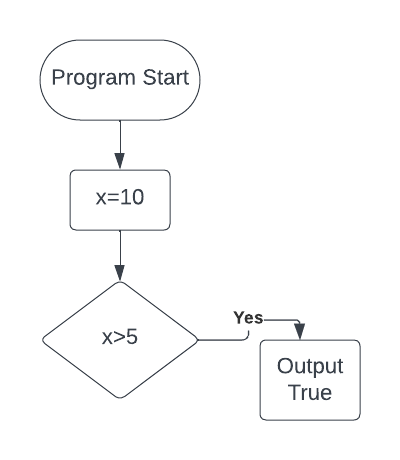
\includegraphics[scale=0.6]{./figures/flowchart1.png}
        \end{center}
    \end{minipage}
    \begin{minipage}[]{0.3\textwidth}
        \begin{center}
            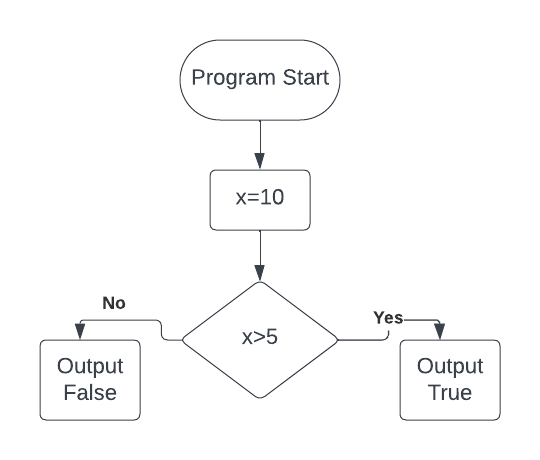
\includegraphics[scale=0.6]{./figures/flowchart2.png}
        \end{center} 
    \end{minipage}
    \begin{minipage}[]{0.3\textwidth}
        \begin{center}
            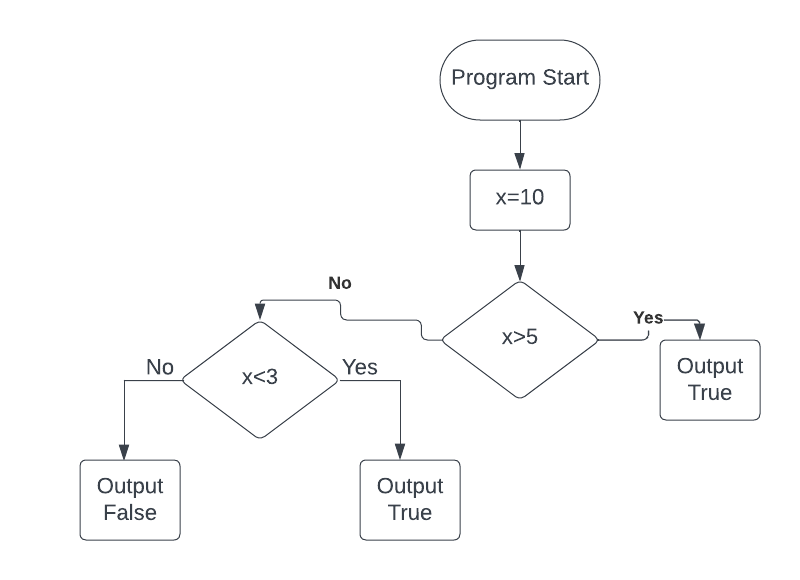
\includegraphics[scale=0.5]{./figures/flowchart3.png}
        \end{center} 
    \end{minipage}


    \bigbreak \noindent 
    \subsection{The Conditional Operator (Ternary)} 
    \bigbreak \noindent 
    \begin{concept}
 You can use the \textbf{conditional operator} to create short expressions that work like if/else statements. The general syntax is as follows:
	\end{concept}
    \smallbreak \noindent
    \line(1,0){490}
    \begin{minted}{cpp}
                            ( condition ) ? Statement_if_true :  statement_if_false
    \end{minted}
    \line(1,0){490}
    \bigbreak \noindent 
    For example:
    \smallbreak \noindent
    \line(1,0){490}
    \begin{minted}[linenos]{cpp}
( x < 0 ) ? y = 10 : z = 20;  

// Equivalent To
if (x < 0) {
    y = 10;
}else {
    z = 20;
}
    \end{minted}
    \line(1,0){490}

    \pagebreak \bigbreak \noindent 
    \subsection{Switch}
    \bigbreak \noindent 
    \begin{concept}
 The \textbf{switch} statement lets the value of a variable or an expression determine where the program will branch. IMPORTANT: Switch can \textbf{ONLY} be used for integers or characters
	\end{concept}
    \bigbreak \noindent 
    The general syntax for the switch statement is as follows:
    \bigbreak \noindent 
    \line(1,0){490}
    \begin{minted}[linenos]{cpp}
switch (value){
    case some_case:
        statements;
        break

    case some_other_case:
        statements;
        break

    default:
        cout << "Cases not matched";
}
    \end{minted}
    \line(1,0){490}
    \bigbreak \noindent 
    \nt{With switch, if we have a default block, it is important that we have a \textbf{break} statement in each case block, say a case is matched and we enter into the block, once the program exits the case block, it will continue on with the rest of the cases. Thus, the default will be triggered.}
    \bigbreak \noindent 
    Here is an example of switch:
    \bigbreak \noindent 
    \line(1,0){490}
    \begin{minted}[linenos]{cpp}
const int x = 10;

switch (x) {
    case 5:
        std::cout << "5";
        break

    case 10:
        std::cout << "10";

    default:
        std::cout << "No Match";
}
    \end{minted}
    \line(1,0){490}
    \bigbreak \noindent 
    \nt{The switch statement in C++ expects constant integral expressions for its case labels. In other words, the value for each case must be known at compile time and cannot be a variable or an expression that involves variables.}

    \pagebreak \bigbreak \noindent 
    \section{\LARGE The While Loop}
    \bigbreak \noindent 
    The general syntax for the C++ while loop is as follows:
    \bigbreak \noindent 
    \line(1,0){490}
    \begin{minted}[linenos]{cpp}
while (expression)
    statement;
// or
while (expression) {
    statements;
}
    \end{minted}
    \line(1,0){490}
    \bigbreak \noindent 
    \begin{minipage}[]{0.47\textwidth}
        Let's take a look a flowchart that describes a while loop:
    \end{minipage}
    \begin{minipage}[]{0.47\textwidth}
        \incfig{while}
    \end{minipage}
    \bigbreak \noindent 
    \nt{The while loop is know as a \textbf{pretest loop}, this is because its nature of testing the condition \textit{before} each iteration}

    \pagebreak \bigbreak \noindent 
    \section{\LARGE The Do-While Loop}
    \bigbreak \noindent 
    \begin{concept}
 The do while loop is a \textbf{posttest} loop which means its expression is tested after each iteration. Below is the general syntax for the do-while loop in C++:
	\end{concept}
    \bigbreak \noindent 
    \line(1,0){490}
    \begin{minted}[linenos]{cpp}
do 
    statement
while (expression);

// or 

do {
    statements;
} while (expression);
    \end{minted}
    \line(1,0){490}
    \bigbreak \noindent 
    \begin{minipage}[]{0.47\textwidth}
        Let's take a look at a simple flowchart that describes this concept.
    
    \end{minipage}
    \begin{minipage}[]{0.47\textwidth}
        \incfig{dowhlie3}
    \end{minipage}

    \pagebreak \bigbreak \noindent 
    \section{\LARGE The for loop}
    \bigbreak \noindent 
    \begin{concept}
 There are two types of loops, \textbf{conditional loops} and \textbf{count-controlled loops}. The for loop demonstrates a count-controlled loop, this type of loop is ideal for performing a known number of iterations.
	\end{concept}
    \bigbreak \noindent 
    The general syntax for the for loop is as follows
    \bigbreak \noindent 
    \line(1,0){490}
    \begin{minted}[linenos]{cpp}
for (initialization; test; update)  
    statement;

// or

for (initialization; test; update) { 
    statements;
}
    \end{minted}
    \line(1,0){490}

    \bigbreak \noindent 
    \nt{It is valid syntax to execute more than one statement in the initialization expression and the update expression. Additionally, the initialization stage of the for loop declaration if has already been preformed or if no Initialization is needed.}
    \bigbreak \noindent 
    below is an example of a for loop without the initialization stage.
    \bigbreak \noindent 
    \line(1,0){490}
    \begin{minted}[linenos]{cpp}
int x=0;
for ( ; x < 10; ++x) {
    statements;
}

    \end{minted}
    \line(1,0){490}
    \bigbreak \noindent 
    You may also omit the update stage of the for loop header if it will be preformed elsewhere in the loop body. In fact, you can even go as far as omitting all three expressions in loops parenthesis.

    \pagebreak \bigbreak \noindent 
    \section{\LARGE Using Files for Data Storage}
    \bigbreak \noindent 
    \begin{concept}
 When a program needs to save data for later use, it writes the data in a file. The data can then be read from the file at a later time.
	\end{concept}
    \bigbreak \noindent 
    \subsection{File Access Methods}
    \bigbreak \noindent 
    There are two general ways to access data stored in a file: \textit{sequential access} and \textit{direct access}. When you work with \textit{sequential-access file}, you access data from the beginning of the file to the end of the file.
    \bigbreak \noindent 
    When you work with a \textit{direct-access file}, you can jump to any piece  of data within the file without reading the data that comes before it.
    \bigbreak \noindent 
    \subsection{Setting up a program for file input/output}
    \bigbreak \noindent 
    In order for us to use file stream objects, we must include <fstream>.
    \bigbreak \noindent 
    \line(1,0){490}
    \begin{minted}[linenos]{cpp}
#include <fstream>
    \end{minted}
    \line(1,0){490}
    \bigbreak \noindent 
    \subsection{File Stream Objects}
    \bigbreak \noindent 
    In order for a program to work with a file on the computer's disk, the program must create a file stream object in memory. A \textit{file stream object} is an object that is associated with a specific file and provides a way for the program to work with that file. 
    \bigbreak \noindent 
    \textbf{File Stream Objects:}
    \begin{itemize}
        \item ofstream: we use this object when we want to create a file and write to it
        \item ifstream: we use this object when we want to open an existing file and read from it
        \item fstream: we use this object when we want to either read or write to a file
    \end{itemize}

    \pagebreak \bigbreak \noindent 
    \subsection{Creating a file object and opening a file}
    \bigbreak \noindent 
    Before data can be written to or read from a file, the following things must happen:
    \begin{itemize}
        \item A file stream object must be created
        \item The file must be opened and linked to the file stream object
    \end{itemize}
    \bigbreak \noindent 
    The following example shows how to open a file for input (reading):
    \bigbreak \noindent 
    \line(1,0){490}
    \begin{minted}[linenos]{cpp}
std::ifstream inputfile;
inputfile.open("filename.txt");

// Or just
std::ifstream inputfile("filename.txt");

// To read from the file... (assuming there are 2 lines of text)

std::string line1, line2;

inputfile >> line1;
cout << line1;

inputfile >> line2;
cout << line2;
    \end{minted}
    \line(1,0){490}
    \bigbreak \noindent 
    The following example shows how to open a file for output (writing):
    \bigbreak \noindent 
    \line(1,0){490}
    \begin{minted}[linenos]{cpp}
std::ofstream outputfile;
outputfile.open("filename.txt");

// Or just
std::ofstream outputfile("filename.txt");

// To write to the file...
outputfile << "Some text \n";

// This...
string a{" "};
std::ofstream file("./myfile2");

if (file) {
    while (cin >> a && a!="q") {
        file << a << endl;
    }
}

file.close();
    \end{minted}
    \line(1,0){490}

    \bigbreak \noindent 
    \subsection{Closing a file}
    \bigbreak \noindent 
    To close a file we write:
    \bigbreak \noindent 
    \line(1,0){490}
    \begin{minted}[linenos]{cpp}
fileobject.close()
    \end{minted}
    \line(1,0){490}

    \pagebreak \bigbreak \noindent 
    \subsection{Reading from a file with an unknown number of lines}
    \bigbreak \noindent 
    We we use the >> operator to read from a file, it will return either 0 1 depending on if there was any content to read. Thus, we can use a while loop to avoid any errors.
    \bigbreak \noindent 
    \line(1,0){490}
    \begin{minted}[linenos]{cpp}
while (inputfile >> line){
    cout << line << endl;
}
    \end{minted}
    \line(1,0){490}

    \bigbreak \noindent 
    \subsection{Testing for file open errors}
    \bigbreak \noindent 
    Under certain circumstances, the open member function will not work. For example, the following code will fail if the file info.txt does not exist:
    \bigbreak \noindent 
    \line(1,0){490}
    \begin{minted}[linenos]{cpp}
ifstream inputfile;
inputfile.open("info.txt");
    \end{minted}
    \line(1,0){490}
    \bigbreak \noindent 
    To circumvent this problem, we can use a if statement to check if the file has been opened successfully:
    \bigbreak \noindent 
    \line(1,0){490}
    \begin{minted}[linenos]{cpp}
ifstream inputfile("info.txt");
if (inputfile){
    statements;
}

// Or
if (inputfile.fail()) {
    cout << "failed";
}
    \end{minted}
    \line(1,0){490}

    \pagebreak \bigbreak \noindent 
    \section{\LARGE rvalues and lvalues}
    \bigbreak \noindent 
    In C++, values are categorized as either lvalues or rvalues, which play a fundamental role in understanding expressions, value categories, and reference binding in the language.
    \bigbreak \noindent 
    Here's a simplified explanation:

    \bigbreak \noindent 
    \subsection{rvalue (right value):}
    \bigbreak \noindent 
    \begin{enumerate}
        \item \textbf{Temporary} rvalues often represent temporary values that don't have a specific location in memory (i.e., you can't take their address in a straightforward manner). They are typically values that you can't assign to, like a temporary result of an expression.
        \item \textbf{Examples:}
        \begin{itemize}
            \item Literals: 5, true, 'a'
            \item Results of most expressions: x + y, std::move(x)
        \end{itemize}
    \item \textbf{Binding:} You can't bind an rvalue to a regular (lvalue) reference (T\&). However, C++11 introduced rvalue references (T\&\&) which can bind to rvalues. This is fundamental for move semantics and perfect forwarding.
    \end{enumerate}

    \bigbreak \noindent 
    \subsection{lvalue}
    \bigbreak \noindent 
    \begin{enumerate}
        \item \textbf{Location:} An lvalue represents an object that occupies a specific, identifiable location in memory. You can think of lvalues as "things with a name."
        \item \textbf{Examples:}
            \begin{itemize}
                \item Variables: int x;
                \item Dereference of a pointer: *p
                \item Array subscript: arr[5]
            \end{itemize}
        \item \textbf{Binding:} An lvalue can be bound to an lvalue reference (T\&).
        
    \end{enumerate}







    \pagebreak \bigbreak \noindent 
    \section{\LARGE Breaking and Continuing a loop}
    \bigbreak \noindent 
    \begin{concept}
 The \textbf{break} statement causes a loop to terminate early. The \textbf{continue} statement causes it to stop the current iteration and jump to the next one.
	\end{concept}

    \pagebreak \bigbreak \noindent 
    \section{\LARGE Functions}
    \bigbreak \noindent 
    Functions in c++ are pretty simple, here is an example:
    \bigbreak \noindent 
    \line(1,0){490}
    \begin{minted}[linenos]{cpp}
void myfunc() {
    statements;

}
int main(int argc, const char *argv[]){ myfunc(); return EXIT_SUCCESS; }
    \end{minted}
    \line(1,0){490}
    \bigbreak \noindent 
    Where the type before the function identifier is the value that the function shall return.
    \bigbreak \noindent 
    \subsection{Function prototypes (function declarations)}
    \bigbreak \noindent 
    \begin{concept}
 A function prototype eliminates the need to place a function definition before all calls to the function.
	\end{concept}
    \bigbreak \noindent 
    Example:
    \bigbreak \noindent 
    \line(1,0){490}
    \begin{minted}[linenos]{cpp}
void foobar();

void foobar() {
    statements;

}
int main(int argc, const char *argv[]){ foobar(); return EXIT_SUCCESS; }
    \end{minted}
    \line(1,0){490}
    \bigbreak \noindent 
    \nt{Function definitions can be placed below \textit{main}, just prototype them above \textit{main}}
    \bigbreak \noindent 
    And we can add some parameters:
    \bigbreak \noindent 
    \line(1,0){490}
    \begin{minted}[linenos]{cpp}
std::string foobar(std::string name) {
    return "Hello " + name;
}  

int main(int argc, const char *argv[]){ cout << foobar("nate") << endl; } // Hello nate 
    \end{minted}
    \line(1,0){490}

    \pagebreak \bigbreak \noindent 
    \subsection{Static locals}
    \bigbreak \noindent 
    Sometimes we don't want a local variable to be destroyed after the function call completes, in this case we can use the static keyword before the type in our variable declarations
    \bigbreak \noindent 
    \line(1,0){490}
    \begin{minted}[linenos]{cpp}
int foobar() { static int num; return num++; }

int main(int argc, const char *argv[]) {
    std::cout << foobar() << std::endl; // 0
    std::cout << foobar() << std::endl; // 1
    std::cout << foobar() << std::endl; // 2

    return EXIT_SUCCESS;
}
    \end{minted}
    \line(1,0){490}

    \bigbreak \noindent 
    We can also do default values, but these are trivial.

    \bigbreak \noindent 
    \subsection{PREREQ - Reference variables}
    \bigbreak \noindent 
    \begin{concept}
 A reference variable in C++ is an alias, or an alternative name, for an already existing variable. Once a reference is initialized to a variable, either the variable name or the reference name can be used to refer to the variable. Reference variables must be initialized, they cannot just be declared.
	\end{concept}
    \bigbreak \noindent 
    Example:
    \bigbreak \noindent 
    \line(1,0){490}
    \begin{minted}[linenos]{cpp}
int a = 12;
int &b = a; 

cout << a << " " << b << endl; // 12 12

a = 15;
cout << a << " " << b << endl; // 15 15

b = 20; 
cout << a << " " << b << endl; // 20 20

    \end{minted}
    \line(1,0){490}

    \pagebreak \bigbreak \noindent 
    \subsection{Using reference variables as parameters}
    \bigbreak \noindent 
    \begin{concept}
 When used as parameters, reference variables allow a function to access the parameters original arguments. Changes to the parameter are also made to the arguments.
	\end{concept}
    \bigbreak \noindent 
    Example:
    \bigbreak \noindent 
    \line(1,0){490}
    \begin{minted}[linenos]{cpp}
int foobar(int &refvar) { refvar *= 2; return refvar; }

int main(int argc, const char *argv[]) {
    
    int num = 5;

    cout << foobar(num) << endl;  // 10
    cout << foobar(num) << endl;  // 20

    return EXIT_SUCCESS;
}
    \end{minted}
    \line(1,0){490}
    
    \bigbreak \noindent 
    \nt{You cannot pass lvalues to a function that takes a reference variable.}
    \bigbreak \noindent 

    \pagebreak \bigbreak \noindent 
    \subsection{Overloading Functions}
    \bigbreak \noindent 
    \begin{concept}
 Two or more functions can have the same name, as long as their parameters are different.
	\end{concept}
    \bigbreak \noindent 
    Example:
    \bigbreak \noindent 
    \line(1,0){490}
    \begin{minted}[linenos]{cpp}
int foobar(int x, int y) { return x + y; }

int foobar(int x, int y, int z) { return x + y + z; }

int main(int argc, const char *argv[]) {

    cout << foobar(1,2) << endl;
    cout << foobar(1,2,3) << endl;

    return EXIT_SUCCESS;
}
    \end{minted}
    \line(1,0){490}

    \bigbreak \noindent \bigbreak \noindent 
    \subsection{The exit() function}
    \bigbreak \noindent 
    \begin{concept}

	\end{concept}
    \bigbreak \noindent 
    The \textbf{exit()} function causes a program to terminate, regardless of which function or control mechanism is executing.
    \bigbreak \noindent 
    \nt{the exit() function is defined in the cstdlib header}
    \bigbreak \noindent 
    The exit() function must be passed a integer value, usually 0 (EXIT\_SUCCESS), or 1 (EXIT\_FAILURE). We can also just pass the constants EXIT\_SUCCESS/EXIT\_FAILURE, (these constants are defined within cstdlib)
    Example:
    \bigbreak \noindent 
    \line(1,0){490}
    \begin{minted}[linenos]{cpp}
exit(0);
exit(EXIT_SUCCESS);

exit(1);
exit(EXIT_FAILURE)
    \end{minted}
    \line(1,0){490}

    \pagebreak \bigbreak \noindent 
    \subsection{Stubs and Drivers}
    \bigbreak \noindent 
    \begin{concept}
 A \textbf{stub} is a \textit{dummy} function that is called instead of the actual function it represents. It usually displays a test message acknowledging that it was called, and nothing more.
	\end{concept}
    \bigbreak \noindent 
    Example:
    \bigbreak \noindent 
    \line(1,0){490}
    \begin{minted}[linenos]{cpp}
int foobar(int x) {
    std::cout << "Function foobar was called with integer argument " 
    << x 
    << std::endl;
}
    \end{minted}
    \line(1,0){490}
    \bigbreak \noindent 
    This allows for debugging by making sure the function was called at the correct time and with the correct arguments.
    \bigbreak \noindent 
    \begin{concept}
 A \textbf{driver} is a program that tests a function by simply calling it. If the function accepts arguments, the driver passes test data.
	\end{concept}

    \pagebreak \bigbreak \noindent 
    \section{\LARGE Arrays and Vectors}
    \bigbreak \noindent 
    \subsection{Arrays}
    \bigbreak \noindent 
    \begin{concept}
 An array allows you to store and work with multiple values of the same data type. An arrays size declaration must be a constant integer expression with a value greater than or equal to zero. The amount of memory that the array uses depends on the array's data type and the number of elements.
	\end{concept}
    \bigbreak \noindent 
    Example:
    \bigbreak \noindent 
    \line(1,0){490}
    \begin{minted}[linenos]{cpp}
int arr[3]; // array of 3 integer elements
double arr[6]; // array of 6 double elements
int myarr[3] = {1,2,3};

// Getting the elements of an array
std::cout << myarr[0]; // Outputs first value (1)
    \end{minted}
    \line(1,0){490}
    \bigbreak \noindent 
    \nt{Arrays are defined with braces}
    \bigbreak \noindent 

   \bigbreak \noindent 
   \subsection{Partial array initialization}
   \bigbreak \noindent 
   We can also only initialize part of an array. In the case of an integer array, the elements that we do not define will be set to zero. Other cases depend on the data type used.
   \bigbreak \noindent 
   \line(1,0){490}
   \begin{minted}[linenos]{cpp}
int arr[5] = {1,2,3}; // {1,2,3,0,0}
   \end{minted}
   \line(1,0){490}

   \bigbreak \noindent 
   \subsection{Implicit array sizing}
   \bigbreak \noindent 
   Its possible to define an array without specifying a size, as long as we provide an initialization list, c++ will automatically make the array large enough to hold all of the initialization values.

   \bigbreak \noindent 
   \subsection{Bound violation}
   \bigbreak \noindent 
   If we try to add values to a function without any remaining space, the program will crash.

   \pagebreak \bigbreak \noindent 
   \subsection{The range based for loop}
   \bigbreak \noindent 
   \begin{concept}
 The \textbf{range-base for loop} is a loop that iterates once for each element in an array.
	\end{concept}
   \bigbreak \noindent 
   Example:
   \bigbreak \noindent 
   \line(1,0){490}
    \begin{minted}[linenos]{cpp}
int lastindex;
lastindex = (sizeof(arr) / sizeof(arr[0])-1);
for (int i: arr)  {
    if (i != arr[lastindex]) {
        cout << i << ",";
    } else {
        cout << i;
    }
}
   \end{minted}
   \line(1,0){490}

   \subsection{Modifying an array with a range-based for loop}
   \bigbreak \noindent 
   We can declare the range variable as a reference. This way, any change made to \textit{i} will be reflected in our array.
   \bigbreak \noindent 
   \line(1,0){490}
   \begin{minted}[linenos]{cpp}
int arr[3] = {1,2,3};

for (int &i: arr)  {
    i = 5;
}

for (int i : arr) cout << i << " "; // 5 5 5
   \end{minted}
   \line(1,0){490}

   \bigbreak \noindent 
   \subsection{Thou shall not assign}
   \bigbreak \noindent 
   It is crucial to understand  that we can not simply assign an array to some other array variable. The only way to copy over the array to a new variable is to use a loop. Whenever we refer to an array by just its identifier, we are only referring to its \textit{beginning memory address}.
   \bigbreak \noindent 
   A corollary to this concept would lead to the conclusion that we will also not be able to print the contents of an array by:
   \bigbreak \noindent 
   \line(1,0){490}
   \begin{minted}[linenos]{cpp}
int arr[5] = {1,2,3,4,5};
std::cout << arr << std::endl;

   \end{minted}
   \line(1,0){490}
   \bigbreak \noindent 
   This will only display the arrays \textbf{memory address}, we must use a loop to display the contents.

   \pagebreak \bigbreak \noindent 
   \subsection{Getting the size of an array}
   \bigbreak \noindent 
   To get the size of the array, we can use the \textit{sizeof()} function. The way this works is we get the size of the entire array, and then divide by the size of any element.
   \bigbreak \noindent 
    \line(1,0){490}
    \begin{minted}[linenos]{cpp}
int arr[3] = {1,2,3};
std::cout << sizeof(arr) / sizeof(arr[0]) << std::endl;  // 3

// We can also get the last index position by subtracting one
    std::cout << sizeof(arr) / sizeof(arr[0]) - 1 << std::endl;  // 3
    \end{minted}
    \line(1,0){490}
    \bigbreak \noindent 

    \bigbreak \noindent 
    \subsection{Arrays as function arguments}
    \bigbreak \noindent 
    \begin{concept}
  To pass an array as an argument to a function, pass the name of the array. When we pass an array to a function, we are passing a reference to the array, this means any changes to the array in the function will be reflected to the array we passed.
	\end{concept}
    \bigbreak \noindent 
    \line(1,0){490}
    \begin{minted}[linenos]{cpp}
int main(int argc, const char *argv[]) {

    const int SIZE = 3;
    int myarr[3] = {1,2,3};

    for (int i: myarr) cout << i << endl; // 1 2 3

    foobar(myarr, SIZE);

    for (int i: myarr) cout << i << endl; // 2 3 4



    return EXIT_SUCCESS;
}

void foobar(int arr[], int size) {

    for ( int i=0; i < size; ++i ) {
        arr[i]++;
    }


}
    \end{minted}
    \line(1,0){490}

    \bigbreak \noindent 
    \nt{If we do not wish for a function to make any changes to the array argument, we must declare it as const in the function parameters.}

    \pagebreak \bigbreak \noindent 
    \subsection{2D array (matrix)}
    \bigbreak \noindent 
    \begin{concept}
 A two-dimensional array is like sereval identical arrays put together. It is useful for storing multiple sets of data. In mathematics, this type of concept would be called a \textbf{matrix}
	\end{concept}
    \bigbreak \noindent 
    \begin{minipage}[]{0.47\textwidth}
    Consider the arrays:
    \begin{center}
        $A = \{a_{1}, a_{2}, a_{3}\} $ \\
        $a_{1} = \{1,2,3\} $ \\
        $a_{2} = \{4,5,6\} $ \\
        $a_{3} = \{7,8,9\} $ \\
    \end{center}
    \end{minipage}
    \begin{minipage}[]{0.47\textwidth}
    Then we have:
    \begin{align*}
        \begin{bmatrix}
            1 & 2 & 3 \\
            4 & 5 & 6 \\
            7 & 8 & 9
        \end{bmatrix}
    .\end{align*}
    \end{minipage}
    \bigbreak \noindent 
    So in C++, this would be:
    \bigbreak \noindent 
    \line(1,0){490}
    \begin{minted}[linenos]{cpp}
int arr[3][3] = {{1,2,3}, {4,5,6}, {7,8,9}};
int arr[3][3] = {
                {1,2,3},
                {4,5,6},
                {7,8,9}
            };
// and we can index a matrix with
arr[row number][column number];
std::cout << arr[0][0];  // 1
    \end{minted}
    \line(1,0){490}
    \bigbreak \noindent 
    The way we can output all elements of this matrix would look something like:
    \bigbreak \noindent 
    \begin{minipage}[t]{0.47\textwidth}
    \bigbreak \noindent 
    \line(1,0){490}
    \begin{minted}[linenos]{cpp}

    const int SIZE = 3;
    int arr[3][3] = {
                {1,2,3},
                {4,5,6},
                {7,8,9}
            };

    for (int i{0}; i < SIZE; ++i) {
        for (int j{0}; j < SIZE; ++j) {
            cout << arr[i][j] << " ";
        } 
        cout << endl;
    }
    \end{minted}
    \line(1,0){490}
    \end{minipage}
    \hspace{0.2in} 
    \begin{minipage}[t]{0.47\textwidth}
\bigbreak \noindent 
\line(1,0){490}
\begin{minted}[linenos]{cpp}
    const int ROW_SIZE = 3;
    const int COLUMN_SIZE = 4;
    int arr[ROW_SIZE][COLUMN_SIZE] = {
                {1,2,3},
                {4,5,6,6},
                {7,8,9}
            };

    for (int i{0}; i < ROW_SIZE; ++i) {
        for (int j{0}; j < COLUMN_SIZE; ++j) {
            cout << arr[i][j] << " ";
        } 
        cout << endl;
    }
\end{minted}
\line(1,0){490}
    
    \end{minipage}

    \pagebreak \bigbreak \noindent 
    \subsection{Passing a matrix to a function}
    \bigbreak \noindent 
    Unlike array parameter declarations not needing a size, matrix parameters do.
    \bigbreak \noindent 
    \line(1,0){490}
    \begin{minted}[linenos]{cpp}
const int ROW_SIZE = 3;
const int COLUMN_SIZE = 4;

void foobar(const int arr[][COLUMN_SIZE], int row_size) {
    for (int i{0}; i < row_size; ++i) {
        for (int j{0}; j < COLUMN_SIZE; ++j) {
            cout << arr[i][j] << " ";
        }
        cout << endl;
    }
}

int main(int argc, const char *argv[]) {


    int arr[ROW_SIZE][COLUMN_SIZE] = {
                {1,2,3},
                {4,5,6,6},
                {7,8,9}
            };

    foobar(arr, ROW_SIZE);

    return EXIT_SUCCESS;
}
    \end{minted}
    \line(1,0){490}

    \pagebreak \bigbreak \noindent 
    \subsection{The STL Vector}
    \bigbreak \noindent 
    \textbf{Concept. } The \textit{Standard Template Library} offers a \textbf{vector} data type, which in many ways, is superior to standard arrays.
    \bigbreak \noindent 
    The STL is a collection of data types and algorithms that you may use in your programs. 
    \bigbreak \noindent 
    A \textbf{vector} is a container that can store data. It is like an array in the following ways:
    \begin{itemize}
        \item A vector holds a sequence of values.
        \item A vector stores its elements in a contiguous memory location.
        \item You can use the array subscript operator []
    \end{itemize}

    \bigbreak \noindent 
    \subsection{Defining a vector}
    \bigbreak \noindent 
    \line(1,0){490}
    \begin{minted}[linenos]{cpp}
#include <vector>
std::vector<type> name(size); // size is optional 
// Examples
std::vector<int> a(3); // Vector of ints, size 3 with fill of zeros
std::vector<int> a(3, 2); // Vector of ints, size 3 with fill of twos
std::vector<int> a(othervector) // Copy of some other vector
std::vector<int> b = {1,2,3}; // Vector of ints
std::vector<int> b {1,2,3}; // Vector of ints
std::vector<int> b{1,2,3}; // Vector of ints
    \end{minted}
    \line(1,0){490}
    \bigbreak \noindent 
    \nt{If we declare a size for the vector, we \textbf{cannot} define its elements in the same statement, defining elements of a vector in the same statement in which it's declared automatically defines its size, so manually doing is not only not needed, but will produce an error.}

    \bigbreak \noindent 
    \subsection{Get index position of elements}
    \bigbreak \noindent 
    To get the index position of an element in a vector, we can use the \textbf{at(\textit{pos})} member function.
    \bigbreak \noindent 
    Example:
    \bigbreak \noindent 
    \line(1,0){490}
    \begin{minted}[linenos]{cpp}
std::vector<int> a {1,2,3};
cout << a.at(0); // 1
    \end{minted}
    \line(1,0){490}

    \bigbreak \noindent 
    \subsection{Adding to a vector}
    \bigbreak \noindent 
    To store a value in a vector that does not have a starting size, or that is already full, use the \textbf{push\_back()} member function. This function accepts an element and stores it at the end of the vector.
    \bigbreak \noindent 
    Example:
    \bigbreak \noindent 
    \line(1,0){490}
    \begin{minted}[linenos]{cpp}
std::vector<int> a {1,2,3};
a.push_back(4);
    \end{minted}
    \line(1,0){490}

    \bigbreak \noindent 
    \subsection{Getting the size of a vector}
    \bigbreak \noindent 
    To get the size of a vector, we can use the \textbf{size()} member function.
    \bigbreak \noindent 
    Example:
    \bigbreak \noindent 
    \line(1,0){490}
    \begin{minted}[linenos]{cpp}
std::vector<int> a {1,2,3};
std::cout << size(a) << std::endl;  // 3
    \end{minted}
    \line(1,0){490}

    \bigbreak \noindent 
    \subsection{Removing last element of a vector} 
    \bigbreak \noindent 
    To remove elements from a vector, we can utilize the \textbf{pop\_back()} member function. This function will remove the last element of the vector.
    \bigbreak \noindent 
    Example:
    \bigbreak \noindent 
    \line(1,0){490}
    \begin{minted}[linenos]{cpp}
std::vector<int> a {1,2,3};
a.pop_back(); // Removes the last element (3).
    \end{minted}
    \line(1,0){490}

    \bigbreak \noindent 
    \subsection{Removing elements of a vector }
    \bigbreak \noindent 
    To remove elements:
    \bigbreak \noindent 
    \line(1,0){490}
    \begin{minted}[linenos]{cpp}
std::vector<int> myvec{1,2,3,4};
myvec.erase(myvec.begin() + 1); // Removes the second element (2)
    \end{minted}
    \line(1,0){490}

    \bigbreak \noindent 
    \subsection{Clearing a vector}
    \bigbreak \noindent 
    To clear a vector we can use the \textbf{clear()} member function.
    \bigbreak \noindent 
    Example:
    \bigbreak \noindent 
    \line(1,0){490}
    \begin{minted}[linenos]{cpp}
std::vector<int> a {1,2,3};
a.clear();
    \end{minted}
    \line(1,0){490}

    \bigbreak \noindent 
    \subsection{Detecting an Empty vector}
    \bigbreak \noindent 
    To determine if a vector is empty, we can use the \textbf{empty()} function. This function will return 0 or 1 depending on whether the vector contains any elements.
    \bigbreak \noindent 
    Example:
    \bigbreak \noindent 
    \line(1,0){490}
    \begin{minted}[linenos]{cpp}
std::vector<int> a {1,2,3};
std::vector<int> b;
cout << a.empty(); // 0
cout << b.empty(); // 1
    \end{minted}
    \line(1,0){490}

    \bigbreak \noindent 
    \subsection{Resizing a vector}
    \bigbreak \noindent 
    To resize a vector, we can use the \textbf{resize()} member function.
    \bigbreak \noindent 
    Example:
    \bigbreak \noindent 
    \line(1,0){490}
    \begin{minted}[linenos]{cpp}
std::vector<int> a {1,2,3};
a.resize(5,2); // resize the vector to a total size of 5 elements, filling with 2s.
a.resize(5); // resize the vector to a total size of 5 elements, filling with 0s.
    \end{minted}
    \line(1,0){490}

    \bigbreak \noindent 
    \subsection{Swapping Vectors}
    \bigbreak \noindent 
    To swap the contents of two vectors, we can use the \textbf{swap(\textit{vector})} member function.
    \bigbreak \noindent 
    Example:
    \bigbreak \noindent 
    \line(1,0){490}
    \begin{minted}[linenos]{cpp}
std::vector<int> v1 {1,2,3};
std::vector<int> v2 {4,5,6};

v1.swap(v2);
    \end{minted}
    \line(1,0){490}

    \pagebreak \bigbreak \noindent 
    \section{\LARGE Searching and Sorting Arrays}
    \bigbreak \noindent 
    \begin{concept}
 A search algorithm is a method of locating a specific item in a larger collection of data. This section discusses two algorithms for searching the contents of an array.
	\end{concept}
    \bigbreak \noindent 
    \subsection{The linear search}
    \bigbreak \noindent 
    The linear search is very simple, it uses a loop to sequentially step through an array, starting with the first element.
    \bigbreak \noindent 
    Example:
    \bigbreak \noindent 
    \line(1,0){490}
    \begin{minted}[linenos]{cpp}
int main(int argc, const char *argv[]) {

    const int SIZE = 5;
    int arr[SIZE] = {88,67,5,23,19};

    int target = 5;

    for (int i{0}; i <= SIZE + 1; ++i) {
        if (i == SIZE + 1) {
            cout << "Target not in array" << endl;
        }
        if ( arr[i] == target ) {
            cout << "Target [" << target << "] found at index position " << i << endl;
            break;
        }
    }
    return EXIT_SUCCESS;
}
    \end{minted}
    \line(1,0){490}
    \bigbreak \noindent 
    \line(1,0){490}
    \begin{minted}[linenos]{cpp}
int linearsearch(int arr[], int size, int target) {
    int index{0}, position{-1};
    bool found = false;

    while (index < size && !found) {
        if (arr[index] == target) {
            position = index;
            found = true;
        }
        ++index;
    }
    return position;
}
    \end{minted}
    \line(1,0){490}
    \bigbreak \noindent 
    \pagebreak \bigbreak \noindent 
    One drawback to the linear search is its potential inefficiency, its quite obvious to notice that for large arrays, the linear search will take a long time, if an array has 20,000 elements, and the target is at the end, then the search will have to compare 20,000 elements.
    \bigbreak \noindent 
    \subsection{The binary search}
    \bigbreak \noindent 
    The binary search algorithm is a clever approach to searching arrays. Instead of testing the array's first element, the algorithm starts with the leement in the middle. If that element happens to contain the desired value, then the search is over. Otherwise, the value in the middle element is either greater than or less than the value being searched for. If it is greater, then the desired value (if it is in the array), will be found somewhere in the first half of the array. If it is less, then the desired value, it will be found somewhere in the last half of the array. In either case, half of the array's elements have been eliminated from further searching.
    \bigbreak \noindent 
    \nt{The binary search algorithm requires the array to be sorted.}
    \bigbreak \noindent 
    Example:
    \bigbreak \noindent 
    \line(1,0){490}
    \begin{minted}[linenos]{cpp}
int binarysearch(int arr[], int size, int target) {
    int first{0}, 
        middle,
        last = size -1,
        position{-1};

    bool found = false;

    while (!found && first <= last) {
        middle = (first + last) / 2;
        if (arr[middle] == target) {
            found = true;
            position = middle;
        } else if (target > arr[middle]) {
            first = middle + 1;
        } else {
            last = middle - 1;
        }
    }
    return position;
}
    \end{minted}
    \line(1,0){490}
    \bigbreak \noindent 
    Powers of twos are used to calculate the max number of comparisons the binary search will make on an array. Simply find the smallest power of 2 that is greater than or equal to the number of elements in the array. For example:
    \bigbreak \noindent 
    \begin{minipage}[]{0.47\textwidth}
    \begin{align*}
        n = 50,000 \\
        2^{15} = 32,768 \\
        2^{16} = 65,536
    .\end{align*}
    \end{minipage}
    \begin{minipage}[t]{0.47\textwidth}
        Thus, there are a maximum of 16 comparisons for a array of size 50,000
    \end{minipage}

    \pagebreak \bigbreak \noindent 
    \subsection{Bubble Sort}
    \bigbreak \noindent 
    The bubble sort algorithm makes passes through and compares the elements of the array, certain values "bubble" toward the end of the array with each pass.
    \bigbreak \noindent 
    Example:
    \bigbreak \noindent 
    \line(1,0){490}
    \begin{minted}[linenos]{cpp}
void swap(int &a, int &b) {
    int temp = a;
    a = b;
    b = temp;
}

void bubblesort(int arr[], int size) {

    for (int max = size; max > 0; --max) {
        for (int i{0}; i < size; ++i) {
            if (arr[i] > arr[i + 1]) {
                swap(arr[i], arr[i+1]);
            }
        }
    } 
}
    \end{minted}
    \line(1,0){490}

    \bigbreak \noindent 
    \subsection{Selection Sort}
    \bigbreak \noindent 
    The bubble sort algorithm is simple, but it is ineffective because values move by only one element at a time toward their final destination in the array. The \textit{selection sort algorithm} usually performs fewer swaps because it moves items immediately to their final position in the array. 
    \bigbreak \noindent 
    Example:
    \bigbreak \noindent 
    \line(1,0){490}
    \begin{minted}[linenos]{cpp}
void swap(int &a, int &b) {
    int temp = a;
    a = b;
    b = temp;
}

void selectionsort(int arr[], int size) {


    for(int j=0; j < size; ++j) {
        int &minelement = arr[j];
        for (int k = j+1; k < size; ++k) {
            if ( arr[k] < minelement ) {
                swap(minelement, arr[k]);
            }
        }

    }
}
    \end{minted}
    \line(1,0){490}

    \pagebreak \bigbreak \noindent 
    The selection sort starts with the assumption that the first element is already the smallest, then it scans the array and tries to find a smaller value. If one is found, it moves that element to the front. Once the iteration is complete, we can be sure that the smallest value is at the front and +1 is added to the loop index.

    \pagebreak \bigbreak \noindent 
    \section{\LARGE Pointers}
    \bigbreak \noindent 
    \begin{concept}
 Pointers are variables that store the memory address of a variable, we can use the \& operator to retrieve the address of a variable. Pointers are like references, any changes we make to the variable the holds the pointer, the change will be reflected in the original variable.
	\end{concept}
    \bigbreak \noindent 
    \nt{In order to access the contents of a pointer, we must \textbf{dereference}, more on this later.}
    \bigbreak \noindent 
    Example:
    \bigbreak \noindent 
    \line(1,0){490}
    \begin{minted}[linenos]{cpp}
int a = 12;
int *b; // Initialize pointer  
b = &a; // Get the memory address of a and store in b
cout << b; // Output the memory address
cout << *b; // Output the contents
*b = 15; // Change the value of b, change reflected to a
// We can also put the asterisk next to the type
int* b;
    \end{minted}
    \line(1,0){490}

    \bigbreak \noindent 
    \subsection{Nullptr}
    \bigbreak \noindent 
    It is never a good idea to use an uninitialized pointer, this could mean we are affecting some random memory address. To circumvent this, we can use the bulitin keyword \textit{nullptr}. Assigning a pointer to nullptr means we are assigning it to the address zero. When we do this, we say that the pointer points to "nothing".
    \bigbreak \noindent 
    \line(1,0){490}
    \begin{minted}[linenos]{cpp}
int* b = nullptr;
    \end{minted}
    \line(1,0){490}
    \bigbreak \noindent 
    \nt{If we try to deference the contents of a nullptr, we will get \textbf{address boundary error} at runtime}

    \pagebreak\bigbreak \noindent 
    \subsection{Arrays as pointers}
    \bigbreak \noindent 
    \begin{concept}
 Array names can be used as constant pointers, and pointers can be used as array names.
	\end{concept}
    \bigbreak \noindent 
    We have already discussed that referencing an array without the subscript operator returns the address of the beginning of the array. Thus, we can conclude that an array is just a \textit{pointer} to the first element.
    \bigbreak \noindent 
    If we deference an array, we can get access to the first element.
    \bigbreak \noindent 
    \line(1,0){490}
    \begin{minted}[linenos]{cpp}
int arr[3] = {1,2,3};
cout << *arr << endl; // 1
    \end{minted}
    \line(1,0){490}
    \bigbreak \noindent 
    We can gain access to the other elements via some simply arithmetic:
    \bigbreak \noindent 
    \line(1,0){490}
    \begin{minted}[linenos]{cpp}
int arr[3] = {1,4,3};
cout << *(arr+1); // 4
    \end{minted}
    \line(1,0){490}
    \bigbreak \noindent 
    We we add one to \textit{arr}, we are actually adding 1 multiplied by the size of the data type that we are trying to access. This allows us to change the address of the first element to the address of the second.
    \bigbreak \noindent 
    Therefore, we can generalize:
    \bigbreak \noindent 
    \line(1,0){490}
    \begin{minted}[linenos]{cpp}
arr[index] = *(arr + index)
    \end{minted}
    \line(1,0){490}

    \bigbreak \noindent 
    We can assign pointers to arrays
    \bigbreak \noindent 
    \line(1,0){490}
    \begin{minted}[linenos]{cpp}
int arr[3] = {1,2,3};
int* b = arr;
cout << *b << endl; // 1
for (int i{0}; i < 3; ++i) {
    cout << b[i] << endl;
}
    \end{minted}
    \line(1,0){490}

    \pagebreak \bigbreak \noindent 
    \subsection{Pointers as Function Parameters}
    \bigbreak \noindent 
    We can also declare pointer parameters in functions, giving the function access to the original variable, much like reference
    \bigbreak \noindent 
    \line(1,0){490}
    \begin{minted}[linenos]{cpp}
void foobar(int* pt) {
    *pt = 5;
}

int a = 10;
foobar(&a); // Changes a to the value 5

    \end{minted}
    \line(1,0){490}

    \bigbreak \noindent 
    \subsection{Pointers to constants}
    \bigbreak \noindent 
    Sometimes, it is necessary to pass the address of a const item into a pointer. When this is the case, the pointer must be defined as a pointer to a const item.
    \bigbreak \noindent 
    \line(1,0){490}
    \begin{minted}[linenos]{cpp}
const int* b; 
const int *b;
    \end{minted}
    \line(1,0){490}
    \bigbreak \noindent 
    \nt{It should be noted that the keyword const is referring to the thing that $b$ is pointing to, not $b$ itself. Furthermore, it is crucial that we have the const modifier on line 2, if we are trying to point to a constant, then this is required. This does not mean the thing we are trying to point to needs the const qualifier for line 2 to be valid. lastly, because $b$ is a pointer to a const, the compiler will not allow us to write code that changes the thing that $b$ points to.}
    \bigbreak \noindent 

    \pagebreak \bigbreak \noindent 
    \subsection{Constant Pointers}
    \bigbreak \noindent 
    We can also use the const key word to define a constant pointer. Here are the differences:
    \begin{itemize}
        \item A pointer to a const points to a constant item. The data that the pointer points to cannot change, but the pointer itself can change. 
        \item With a const pointer, it is the pointer itself that is constant.  Once the pointer is initialized with an address, it cannot point to anything else.
    \end{itemize}
    \bigbreak \noindent 
    Example:
    \bigbreak \noindent 
    \line(1,0){490}
    \begin{minted}[linenos]{cpp}
int* const ptr;
int *const ptr;
    \end{minted}
    \line(1,0){490}

    \bigbreak \noindent 
    \subsection{Both pointer to constant and constant pointer}
    \bigbreak \noindent 
    \line(1,0){490}
    \begin{minted}[linenos]{cpp}
const int* const ptr;
const int *const ptr;
    \end{minted}
    \line(1,0){490}

    \bigbreak \noindent 
    \subsection{Prereq - Static vs Dynmaic memory allocation}
    \bigbreak \noindent 
    There are different types of memory allocation in a C++ program. By default, creating variables will utilize "static memory allocation", this is where variables are created on the "stack". The stack is a region of memory where local variables, function parameters, return addresses, and control flow data are stored. It operates in a Last-In-First-Out (LIFO) manner.
    \bigbreak \noindent 
    When a function is called, a new "stack frame" is pushed onto the stack. This frame contains the function's local variables, parameters, and the return address.
    When the function returns, its stack frame is popped off, and the stack pointer moves back to the previous frame.
    The stack grows and shrinks automatically as functions are called and return.
    \bigbreak \noindent 
    \textbf{Characteristics:}
    \begin{itemize}
        \item \textbf{Automatic Memory Management:} Memory allocation and deallocation on the stack are automatic. When a function exits, its local variables are automatically deallocated.
        \item \textbf{Speed:} Stack operations (push and pop) are very fast.
        \item \textbf{Fixed Size:} The stack has a fixed size, determined at the start of the program. If a program uses more stack space than is available (e.g., due to deep or infinite recursion), it will result in a "stack overflow."
    \end{itemize}
    \bigbreak \noindent 
    In constrast to this, we also have \textbf{dynmaic memory allocation}: In has the following characteristics:
    \begin{itemize}
        \item Memory is allocated during runtime.
        \item Uses functions like malloc(), calloc(), realloc(), and new (in C++) to allocate memory.
        \item Requires manual deallocation using functions like free() or delete (in C++).
        \item Memory is allocated on the heap.
        \item The size of the memory allocation can be determined at runtime based on program needs.
    \end{itemize}



    \bigbreak \noindent 
    \subsection{Dynamic Memory Allocation}
    \bigbreak \noindent 
    \begin{concept}
 Variables may be created and destroyed while a program is running.
	\end{concept}
    \bigbreak \noindent 
    In the cases where we don't know how many variables we will need for a program, we can allow a program to create its own variables "on the fly". This is called \textit{dynamic memory allocation} and this is only possible through pointers.
    \bigbreak \noindent 
    To dynamically allocate memory means that a program, while running, asks the computer
to set aside a chunk of unused memory large enough to hold a variable of a specific data
type. Let’s say a program needs to create an integer variable. It will make a request to the
computer that it allocate enough bytes to store an int. When the computer fills this request,
it finds and sets aside a chunk of unused memory large enough for the variable. It then gives
the program the starting address of the chunk of memory. The program can only access the
newly allocated memory through its address, so a pointer is required to use those bytes.

    \bigbreak \noindent 
    The way a C++ program requests dynamically allocated memory is through the new operator. Assume a program has a pointer to an int defined as
    \bigbreak \noindent 
    \line(1,0){490}
    \begin{minted}[linenos]{cpp}
int *ptr = nullptr;
// Then we can do:
ptr = new int;
// A value may be stored in this new variable by dereferencing the pointer:
*ptr = 15;
    \end{minted}
    \line(1,0){490}

    \bigbreak \noindent 
    This statement is requesting that the computer allocate enough memory for a new int variable. The operand of the new operator is the data type of the variable being created. Once the statement executes, ptr will contain the address of the newly allocated memory. Then we store a value in the new variable by dereferencing.
    \bigbreak \noindent 
    Although the statements above illustrate the use of the new operator, there’s little purpose
in dynamically allocating a single variable. A more practical use of the new operator is to
dynamically create an array. Here is an example of how a 100-element array of integers
may be allocated:
\bigbreak \noindent 
\line(1,0){490}
\begin{minted}[linenos]{cpp}
ptr = new int[100];
\end{minted}
\line(1,0){490}
\bigbreak \noindent 
    Once the array is created, the pointer may be used with subscript notation to access it. 

    \bigbreak \noindent 
     it should
release it for future use. The delete operator is used to free memory that was allocated
with new. Here is an example of how delete is used to free a single variable, pointed to
by iptr :
    \bigbreak \noindent 
    \line(1,0){490}
    \begin{minted}[linenos]{cpp}
delete ptr;
ptr = nullptr; // Always set to nullptr after deleting
delete [] ptr; // If ptr points to a dynamically allocated array
ptr = nullptr; // Always set to nullptr after deleting
    \end{minted}
    \line(1,0){490}
    \bigbreak \noindent 
    \nt{Failure to release dynamically allocated memory can cause a program to have a memory leak. Only use pointers with delete that were previously used with new. If you use a pointer with delete that does not reference dynamically allocated memory, unexpected problems could result!}
    \bigbreak \noindent 

    \bigbreak \noindent 
    \subsection{When to use DMA}
    \bigbreak \noindent 
    \begin{enumerate}
        \item Memory Location: The integer is allocated on the heap.
        \item Lifetime: The memory remains allocated until it's explicitly deallocated using delete.
        \item Use Cases:
        \begin{itemize}
            \item Variable Size: When you need data structures of variable size, like linked lists or dynamic arrays.
            \item Long-lived Objects: When you need objects that outlive the function they were created in.
            \item Avoiding Stack Overflow: For large allocations, the stack might not have enough space, leading to stack overflow. In such cases, DMA is preferred.
            \item For Polymorphism: In object-oriented programming, DMA is often used with pointers to base and derived classes to achieve polymorphism.
        \end{itemize}
    \end{enumerate}

    \bigbreak \noindent 
    \subsection{Returning pointers from a function}
    \bigbreak \noindent 
    \begin{concept}
 Functions can return pointers, but you must be sure the item the pointer references still exists.
	\end{concept}
    \bigbreak \noindent 
    We should return  a pointer from a function only if it is:
    \begin{itemize}
        \item A pointer to an item that was passed into the function as an argument.
        \item A pointer to a dynamically allocated chuck of memory
    \end{itemize}

    \bigbreak \noindent 
    \subsection{Smart Pointers}
    \bigbreak \noindent 
    \begin{concept}
 C++ 11 introduces smart pointers, objects that work like pointers, but have the ability to automatically delete dynamically allocated memory that is no longer being used.
	\end{concept}
    \bigbreak \noindent 
    We have three types:
    \begin{itemize}
        \item \textbf{unique\_ptr}: The sole owner of a piece of dynamically allocated memory. 
        \item \textbf{shared\_ptr}: Can share ownership of a piece of dynamically allocated memory. Multiple pointers of the shared\_ptr type can point to the same piece of memory
        \item \textbf{weak\_ptr}: Does not own the memory it points to, and cannot be used to access the memory's contents. Used when the memory pointed to by a shared\_ptr must be referenced without increasing the number of shared\_ptrs that own it.
    \end{itemize}
    \bigbreak \noindent 
    \nt{To use these smart pointers, we must include <memory>}

    \pagebreak \bigbreak \noindent 
    Here is the syntax for a unique pointer:
    \bigbreak \noindent 
    \line(1,0){490}
    \begin{minted}[linenos]{cpp}
unique_ptr<type> name( new type );
// Example
std::unique_ptr<int> a( new int ); // Basic way 
std::unique_ptr<int> a = std::make_unique<int>(15); // Preferred Way (Initialization of 15)
std::unique_ptr<int> a = std::make_unique<int>(); // Preferred Way (initialization of zero)
std::shared_ptr<int> b = a; //  NOT VALID, unique_ptr must be unique
    \end{minted}
    \line(1,0){490}
    \bigbreak \noindent 
    So now we have two entities: a \textbf{unique\_ptr} located on the \textit{stack} and an \textbf{int} located on the \textit{heap}. The unique\_ptr holds the address of the int we created on the heap. Since this is a \textbf{smart pointer}, the integer object will be deleted and the unique pointer that was holding the memory address will be set to nullptr will be deleted and the unique pointer that was holding the memory address will be set to \textbf{nullptr}.
    \bigbreak \noindent 
    A \textbf{shared\_ptr} works via a \textbf{reference counter} maintained in a control block. This mechanism keeps track of how many shared\_ptr instances are pointing to the same object. Once the reference count reaches zero, the managed object is deleted. The control block also tracks weak references and is deallocated when both shared and weak counts reach zero. Here is how we build such object:
    \bigbreak \noindent 
    \line(1,0){490}
    \begin{minted}[linenos]{cpp}
std::shared_ptr<type> identifier( new int ); // Basic Way
std::shared_ptr<type> identifier = std::make_shared<type>(initialization); // Preferred Way
// Example
std::shared_ptr<int> a( new int );
std::shared_ptr<int> a = std::make_shared<int>(10);
std::shared_ptr<int> b = a; // Valid copy
    \end{minted}
    \line(1,0){490}

    \bigbreak \noindent 
    Lastly, we can define a \textbf{weak\_ptr}, we can assign this object to any shared\_ptr object, but the reference count will not be updated.
    \bigbreak \noindent 
    \line(1,0){490}
    \begin{minted}[linenos]{cpp}
std::shared_ptr<int> a = std::make_shared<int>(10);
std::weak_ptr<int> b = a; // Reference count will NOT be updated.
    \end{minted}
    \line(1,0){490}

    \pagebreak \bigbreak \noindent 
    \section{\LARGE Characters, C-Strings and more about the string class}
    \bigbreak \noindent 
    \subsection{Character Testing}
    \bigbreak \noindent 
    The C++ library provides several functions that allaw us to test the value of a character. These functions test a single \textit{char} argument and return either true or false.
    \bigbreak \noindent 
    To use these functions, we must include <cctype>
    \begin{itemize}
        \item isalppha
        \item isalnum
        \item isdigit
        \item islower
        \item isprint
        \item ispunct
        \item isupper
        \item isspace
    \end{itemize}

    \bigbreak \noindent 
    \subsection{Character case conversion}
    \bigbreak \noindent 
    We also have functions for converting characters to uppercase or lowercase.
    \begin{itemize}
        \item toupper
        \item tolower
    \end{itemize}

    \bigbreak \noindent 
    \subsection{C Strings }
    \bigbreak \noindent 
    \begin{concept}
 A C-string is a sequence of characters stored in consecutive memory locations, terminated by a null character. In C++, all string literals are stored in memory as C-Strings. The purpose of  a \textbf{null terminator} is to mark the end of the C-String.
	\end{concept}
    \bigbreak \noindent 
    It's important to realize that a string literal has its own storage location, just like a variable or an array. When a string literal appears in a statement, it's actually its memory address that C++ uses. 

    \pagebreak \bigbreak \noindent 
    \subsection{C-Strings stored in arrays}
    \bigbreak \noindent 
    In C, there is no string class that we can use, so when a C programmer wants to create a string, they must make a char array to house it. The char array must be large enough to house the string, and one extra to hold the null terminator.
    \bigbreak \noindent 
    Here's how we get input from a user and store it in a character array (string)...
    \bigbreak \noindent 
    \line(1,0){490}
    \begin{minted}[linenos]{cpp}
const int SIZE=80;
char a[];
cout << "enter some string: ";
cin.getline(a,SIZE);
    \end{minted}
    \line(1,0){490}
    \bigbreak \noindent 
    Here we are using the cin's member function \textbf{getline()}, where the first argument is where we want to store the input, and the second argument indicates the maximum length of the string, including the null terminator
    \bigbreak \noindent 
    For a summary:
    \bigbreak \noindent 
    \line(1,0){490}
    \begin{minted}[linenos]{cpp}
std::getline(cin, variable) // Used for std::string objects
cin.get(variable) // Used for single characters
cin.getline(variable, size) // Used for character arrays
    \end{minted}
    \line(1,0){490}
    \bigbreak \noindent 
    \nt{We cannot use const char* for user input}

    \bigbreak \noindent 
    \subsection{The Strlen function}
    \bigbreak \noindent 
    To be able to get access to various functios pertaining to C-Strings, we must include <cstring>. Then we can get the size of a string by:
    \bigbreak \noindent 
    \line(1,0){490}
    \begin{minted}[linenos]{cpp}
char name[] = "NATE";
int len;
len = strlen(name);
// These functions are also going to work for the other type of C-String
const char* a;
len = strlen(a);
    \end{minted}
    \line(1,0){490}
    \bigbreak \noindent 
    \nt{The strlen function accepts a pointer to a C-String. Also know that sizeof() will include the null terminator, while strlen will not}


    \pagebreak \bigbreak \noindent 
    \subsection{The strcat Function}
    \bigbreak \noindent 
    The strcat function accepts two pointers to C-Strings as its arguments. The function then concatenates, or appends one string to another.
    \bigbreak \noindent 
    \line(1,0){490}
    \begin{minted}[linenos]{cpp}
char a[20] = "Hello ";
char b[] = "World";
strcat(a,b);

cout << a << endl; // Hello World!

char a[20] = "Hello ";
const char* b = "World";
strcat(a,b);

cout << a << endl; // Hello World!
    \end{minted}
    \line(1,0){490}
    \bigbreak \noindent 
    \nt{With the second example, $a$ cannot be a const char*, and they \textbf{cannot} both be const char*}

    \bigbreak \noindent 
    \subsection{The Strcopy function}
    \bigbreak \noindent 
    Recall that one array cannot be assigned to another array with the = operator. The strcpy function can be used to copy one string to another.
    \bigbreak \noindent 
    \line(1,0){490}
    \begin{minted}[linenos]{cpp}
char a[10];
char b[] = "Hello";
strcpy(a,b);
cout << a << endl; // Hello
// We can also do...
char a[10];
const char* b = "Hello";
strcpy(a,b);
cout << a << endl; // Hello
    \end{minted}
    \line(1,0){490}
    \bigbreak \noindent 
    \nt{For the second example, the thing we are copying to cannot be a const char*}
    \bigbreak \noindent 

    \pagebreak \bigbreak \noindent 
    \subsection{The strncat and strncpy functions}
    \bigbreak \noindent 
    Because the \textbf{strcat} and \textbf{strcpy} functions can possibly overwrite the bounds of an array, they make it possible to write unsafe code. Instead, you should use \textbf{strncat} and \textbf{strncpy} when possible
    \bigbreak \noindent 
    \begin{remark}
       "Overwriting the bounds of an array" refers to accessing or modifying elements of an array outside of its valid index range. In simpler terms, it means trying to read from or write to a location that's not within the array's allocated memory.
    \end{remark}
    \bigbreak \noindent 
    These functions have an additional parameter, it is the maximum number of characters to add to the array. This way, we can define how much space we have left for the string, and pass it to these functions to make sure we don't go out of bounds.
    \bigbreak \noindent 
    \line(1,0){490}
    \begin{minted}[linenos]{cpp}
// strncat
const int SIZE=10;
char a[SIZE] = "Hello, ";
const char* b = "World";

int size_left = SIZE - strlen(a);
strncat(a,b,size_left); // Hello, Wor

// strncpy
const int SIZE=3;
char a[SIZE];
const char* b = "World";

strncpy(a,b,SIZE);

cout << a << endl; // Wor
    \end{minted}
    \line(1,0){490}

    \bigbreak \noindent 
    \subsection{The strstr function}
    \bigbreak \noindent 
    This function searches for a string inside of a string. For instance, it could be used to search for the string "seven" inside the larger string.
    \bigbreak \noindent 
    \line(1,0){490}
    \begin{minted}[linenos]{cpp}
const char* a = "hello world";
const char*b = nullptr;
b = strstr(a, "hello")

cout << b << endl; // hello world
    \end{minted}
    \line(1,0){490}
    \bigbreak \noindent 
    \nt{If the substr is found, it will return the substr and all that comes after it}
    \bigbreak \noindent 

    \pagebreak \bigbreak \noindent 
    \subsection{The strcmp function}
    \bigbreak \noindent 
    This function takes two C-Strings as arguments and returns an integer that indicates how the two strings compare to each other. 
    \begin{itemize}
        \item The result is zero if the two strings are equal on a character-by-character basis.
        \item The result is negative if string1 comes before string2 in alphabetical order.
        \item The result is positive if string1 comes after string2 in alphabetical order.
    \end{itemize}
    \bigbreak \noindent 
    \line(1,0){490}
    \begin{minted}[linenos]{cpp}
const char* a = "Nate";
const char* b = "Warner";

if (!strcmp(a,b)) {
    cout << "These strings are the same" << endl;
} else if (strcmp(a,b) < 0) {
    cout << a << " comes before " << b << " in alphabetical order" << endl;
} else {
    cout << a << " comes after " << b << " in alphabetical order" << endl;
}
    \end{minted}
    \line(1,0){490}

    \bigbreak \noindent 
    \subsection{String/Numeric Conversion Functions}
    \bigbreak \noindent 
    \begin{concept}
 The C++ library provides functions for converting C-Strings and string objects to numeric data types and vice versa.
	\end{concept}
    \bigbreak \noindent 
    \textbf{String to number (C-String)}
    \begin{itemize}
        \item \textbf{atoi:} converts C-String to an integer 
        \item \textbf{atol:} converts C-String to a long integer 
        \item \textbf{atof:} converts C-String to a double
        \item \textbf{}
    \end{itemize}
    \bigbreak \noindent 
    \textbf{String to number (C++ String)}
    \begin{itemize}
        \item \textbf{stoi}: int
        \item \textbf{stol}: long
        \item \textbf{stoul}: unsigned long
        \item \textbf{stoll}: long long
        \item \textbf{stoull}: unsigned long long
        \item \textbf{stof}: float
        \item \textbf{stod}: double
        \item \textbf{stold}: long double
    \end{itemize}
    \bigbreak \noindent 
    \textbf{Number to String (Returns string object)}
    \bigbreak \noindent 
    \begin{itemize}
        \item \textbf{to\_string}
    \end{itemize}

    \pagebreak \bigbreak \noindent 
    \subsection{More on the C++ string (string object)}
    \bigbreak \noindent 
    Unlike C-Strings, there is no need to use a function like strcmp to compare two strings, we can just use the comparison operators. Much like any scripting language you may be familiar with. Not going to go over this stuff, its pretty trivial.

    \bigbreak \noindent 
    \subsection{C++ String definitions}
    \bigbreak \noindent 
    We have various ways to declare and define these string objects.
    \bigbreak \noindent 
    \line(1,0){490}
    \begin{minted}[linenos]{cpp}
string a; // Defines empty string
string a("text"); // Directly call constructor
string a(otherstring) // Copy
string a(otherstring, 5) // Copy, only use the first 5 characters
string a(otherstring,1,5) // Copy, only use characters 1-5
string a('z', 10) // 10 z characters
    \end{minted}
    \line(1,0){490}

    \bigbreak \noindent 
    \subsection{C++ string supported operators}
    \bigbreak \noindent 
    \begin{itemize}
        \item >>
        \item <<
        \item =
        \item +=
        \item +
        \item [] (subscript notation)
    \end{itemize}

    \pagebreak \bigbreak \noindent 
    \section{\LARGE Structures}
    \bigbreak \noindent 
    \begin{concept}
        Abstract data types (ADTs) are data types created by the programmer. ADTs have their own range (or domain) of data and their own sets of operations that may be performed on them. In C++, we can make use of the concept of \textbf{structures} to create these abstract types. 
	\end{concept}

	\bigbreak \noindent 
	\subsection{Abstraction}
	\bigbreak \noindent 
	An \textit{abstraction} is a general model  of something. It is a definition that includes only the general characteristics of an object.

	\bigbreak \noindent 
	\subsection{Abstract data types}
	\bigbreak \noindent 
	An ADT is a data type created by the programmer and is composed of one or more primitive data types. The programmer decides what values are acceptable for the data type, as well as what operations may be performed on the data type. In many cases, the programmer designs his or her own specialized operations.

	\bigbreak \noindent 
	\subsection{Structures}
	\bigbreak \noindent 
	\begin{concept}
	    C++ allows us to group several variables together into a single item known as a structure
	\end{concept}
	\bigbreak \noindent 
	The syntax for a structure is as follows:
	\bigbreak \noindent 
	\line(1,0){490}
	\begin{minted}[linenos]{cpp}
struct tag {
    variable declarations;
    // ... More declarations 
    //     may follow...
};
	\end{minted}
	\line(1,0){490}
	\bigbreak \noindent 
	Suppose we had a payroll system where we have a bunch of variables that are related to each other, then we could define a structure...
	\bigbreak \noindent 
	\line(1,0){490}
	\begin{minted}[linenos]{cpp}
struct Payroll {
    // Members
    int empNumber;
    string name;
    double hours;
    double payrate;
    double grossPay;
};
	\end{minted}
	\line(1,0){490}
	\bigbreak \noindent 
	\nt{Notice the semi colon at the end of the structure definition}

    \bigbreak \noindent 
	It's important to be aware that the structure example in our example does not define a variable. It simply tells the compiler what a payroll structure is made of.
	\bigbreak \noindent 
	Now that we have our structure defined, we can define variables of this type with simple definition statements.
	\bigbreak \noindent 
	\line(1,0){490}
	\begin{minted}[linenos]{cpp}
payroll deptHead;
	\end{minted}
	\line(1,0){490}

	\bigbreak \noindent 
	\subsection{Accessing structure members}
	\bigbreak \noindent 
	\begin{concept}
	    The \textbf{dot operator} allows us to access structure members in a program.
	\end{concept}
	\bigbreak \noindent 
	\line(1,0){490}
	\begin{minted}[linenos]{cpp}
deptHead.empNumber = 475;
	\end{minted}
	\line(1,0){490}

	\bigbreak \noindent 
	\subsection{Initializing a structure (Initialization list)}
	\bigbreak \noindent 
	\begin{concept}
	   The members of a structure variable may be initialized with starting values when the structure variable is defined 
	\end{concept}
	\bigbreak \noindent 
	Consider the example found in the above subsections (Payroll). We can then define a Payroll variable with an initialization list...
	\bigbreak \noindent 
	\line(1,0){490}
	\begin{minted}[linenos]{cpp}
Payroll depthead = {1, "John Doe", 40, 14, 100}
// Alt forms
Payroll depthead{1, "John Doe", 40, 14, 100} 
Payroll depthead{.empNumber = 1, .name="John Doe", .hours=40, .payrate=14, .grossPay100}
Payroll depthead{} // If we had default values
Payroll depthead = {} // If we had default values
	\end{minted}
	\line(1,0){490}

	\pagebreak \bigbreak \noindent 
	\subsection{Arrays of structures}
	\bigbreak \noindent 
	\begin{concept}
	   Arrays of structures can simplify some programming tasks 
	\end{concept}
	\bigbreak \noindent 
	Example:
	\bigbreak \noindent 
	\line(1,0){490}
	\begin{minted}[linenos]{cpp}
struct BookInfo {
    string title;
    string author;
    string publisher;
    double price;
};
const int SIZE = 20;
BookInfo bookList[SIZE];
	\end{minted}
	\line(1,0){490}
	\bigbreak \noindent 
	Here we defined an array, bookList, that has 20 elements. Each element is a BookInfo structure.
	\bigbreak \noindent 
	So we can step through the array to get the contents:
	\bigbreak \noindent 
	\line(1,0){490}
	\begin{minted}[linenos]{cpp}
for (int i=0; i<SIZE; ++i) {
        cout << bookList[i].title << endl;
        cout << bookList[i].author << endl;
        cout << bookList[i].publisher << endl;
        cout << bookList[i].price << endl;
    }
	\end{minted}
	\line(1,0){490}
	\bigbreak \noindent 
	\subsection{Initializing a structure array}
	\bigbreak \noindent 
	To initialize a structure array, we can simply use a initialize list, still considering the above structure example, we can do:
	\bigbreak \noindent 
	\line(1,0){490}
	\begin{minted}[linenos]{cpp}
bookInfo bookList[SIZE] = {
                            {"title1", "author1", "publisher1", 0.1},
                            {"title2", "author2", "publisher2", 0.2},
                            {"title3", "author3", "publisher3", 0.3}
                            };
	\end{minted}
	\line(1,0){490}
	\bigbreak \noindent 

	\pagebreak \bigbreak \noindent 
	\subsection{Nested Structures}
	\bigbreak \noindent 
	Its possible for a structure variable to be a member of another stricter variable.
	\bigbreak \noindent 
	\line(1,0){490}
	\begin{minted}[linenos]{cpp}
struct foo {
    int a;
    int b;
};
struct bar {
    int c;
    foo f1;
};
bar b1;
cout << b1.f1.a;
	\end{minted}
	\line(1,0){490}

	\bigbreak \noindent 
	\subsection{Structures as function arguments}
	\bigbreak \noindent 
	\begin{concept}
	   Structure variables may be passed as arguments to functions 
	\end{concept}
	\bigbreak \noindent 
	\line(1,0){490}
	\begin{minted}[linenos]{cpp}
struct Box {
    double l, w;
};

void Showbox(Box box) {
    cout << box.l << endl << box.w;
}
	\end{minted}
	\line(1,0){490}
	
	\bigbreak \noindent 
	\nt{This is a pretty poor example, but it shows the concept}
	\bigbreak \noindent 

	\pagebreak \bigbreak \noindent 
	\subsection{Constant reference parameters}
	\bigbreak \noindent 
	\begin{concept}
	   Sometimes structures can be quite large. Passing large structures by value can decrease a program's performance. Of course, this can be dangerous, as passing by reference means we can alter the original values. However, we can circumvent this by passing the argument as a constant reference.
	\end{concept}
	\bigbreak \noindent 
	\line(1,0){490}
	\begin{minted}[linenos]{cpp}
struct Box {
    double l, w;
};

void Showbox(const Box& box) {
    cout << box.l << endl << box.w;
}
	\end{minted}
	\line(1,0){490}

	\bigbreak \noindent 
	\subsection{Returning a structure from a function}
	\bigbreak \noindent 
	\begin{concept}
	   A function may return a structure 
	\end{concept}
	\bigbreak \noindent 
	\line(1,0){490}
	\begin{minted}[linenos]{cpp}
struct Circle {
    double radius;
    double diameter;
    double area;

};
Circle getCircleData() {
    Circle temp;

    temp.radius = 10.0;
    temp.diameter = 20.0;
    temp.area = 314.159;
    return temp;
}
myCircle = getCircleData();
	\end{minted}
	\line(1,0){490}

	\pagebreak \bigbreak \noindent 
	\subsection{Pointers to structures}
	\bigbreak \noindent 
	\begin{concept}
	   You may take the address of a structure variable and create variables that are pointers to structures 
	\end{concept}
	\bigbreak \noindent 
	\line(1,0){490}
	\begin{minted}[linenos]{cpp}
Circle myCircle{10.0,20.0,314.159};
Circle* cirptr = nullptr;
cirptr = &mycircle;
// Access
*cirptr.radius = 10; // Doesn't work
(*cirptr).radius = 10; // Works
cirptr->radius = 10; // Special syntax
	\end{minted}
	\line(1,0){490}
	\bigbreak \noindent 

	\bigbreak \noindent 
	\subsection{Dynamically allocating a structure}
	\bigbreak \noindent 
	We can also use a structure pointer and the new operator to dynamically allocate a structure
	\bigbreak \noindent 
	\line(1,0){490}
	\begin{minted}[linenos]{cpp}
Circle *cirptr = nullptr;
cirptr = ( new Circle );
cirptr->radius = 10;
delete cirptr; // Don't forget to delete when your done with it.
	\end{minted}
	\line(1,0){490}
	\bigbreak \noindent 
	\nt{We use the arrow operator to access \textit{pointers to structure objects}, not structures who's members are pointers. To access structure pointer members, we use the syntax in the above syntax labeled "Doesn't work}
	\bigbreak \noindent 
	Lastly, in the case we have a pointer to a structure that contains a pointer member, we need to use a mix of the deference operator \textbf{and} the arrow operator. 
	\bigbreak \noindent 
	\line(1,0){490}
	\begin{minted}[linenos]{cpp}
*ptr->member;
// or
*(*ptr).member;
	\end{minted}
	\line(1,0){490}

	\pagebreak \bigbreak \noindent 
	\subsection{Enumerated data types}
	\bigbreak \noindent 
	\begin{concept}
	   An \textbf{enumerated} data type is a programmer defined data type. It consists of values known as \textbf{enumerators}, which represent integer constants 
	\end{concept}
	\bigbreak \noindent 
	\line(1,0){490}
	\begin{minted}[linenos]{cpp}
enum Day { MONDAY, TUESDAY, WEDNESDAY, THURSDAY, FRIDAY};
cout << MONDAY << endl 
    << TUESDAY << endl 
    << WEDNESDAY << endl 
    << THURSDAY << endl 
    << FRIDAY;
/*
0
1
2
3
4
*/
Day d1; //	We can also create variables of the data type
	\end{minted}
	\line(1,0){490}
	\bigbreak \noindent 
    Because \textit{d1} is a variable of the Day data type, we may assign any of the enumerators MONDAY, TUESDAY, WEDNESDAY, THURSDAY, or, FRIDAY to it.
    \bigbreak \noindent 
    We can think of these enumerators as integer named constants.

    \bigbreak \noindent 
    \subsection{Assigning an integer to an enum variable}
    \bigbreak \noindent 
    We cannot directly assign integer values to enum variables. For example, the following code will produce an error.
    \bigbreak \noindent 
    \line(1,0){490}
    \begin{minted}[linenos]{cpp}
enum Day { MONDAY, TUESDAY, WEDNESDAY, THURSDAY, FRIDAY};
Day d1;
d1 = 10; // Error
    \end{minted}
    \line(1,0){490}
    \bigbreak \noindent 
    Instead, we must cast the integer literal to data of type \textbf{Day}. 
    \bigbreak \noindent 
    \line(1,0){490}
    \begin{minted}[linenos]{cpp}
d1 = static_cast<Day>(10); // Works
    \end{minted}
    \line(1,0){490}

    \pagebreak  \bigbreak \noindent 
    \subsection{Assigning an enumerator to an int variable}
    \bigbreak \noindent 
    We cannot directly assign an integer value to an enum variable. We can, however, directly assign an enumerator to an integer variable.
    \bigbreak \noindent 
    \line(1,0){490}
    \begin{minted}[linenos]{cpp}
int x{0};
x=MONDAY; // Works just fine
    \end{minted}
    \line(1,0){490}
    \bigbreak \noindent 
    We can also assign a variable of an enumerated type to an integer variable
    \bigbreak \noindent 
    \line(1,0){490}
    \begin{minted}[linenos]{cpp}
Day d1 = MONDAY;
int x = d1;
    \end{minted}
    \line(1,0){490}
    \bigbreak \noindent 
    When we don't need to define any variables of the enumerated type, we can actually skip the naming process. When this occurs, we say we have an \textbf{anonymous enumerated type}
    \bigbreak \noindent 
    \subsection{Using math operators to change the value of an enum variable}
    \bigbreak \noindent 
    Again, we must use a cast.
    \bigbreak \noindent 
    \line(1,0){490}
    \begin{minted}[linenos]{cpp}
enum Day { MONDAY, TUESDAY, WEDNESDAY, THURSDAY, FRIDAY};

Day d1 = MONDAY;
d1 = d1 + 1; // Error
d1 = static_cast<Day>(d1 + 1); // Correct
    \end{minted}
    \line(1,0){490}

    \bigbreak \noindent 
    \subsection{Using an enum variable to step through an array's elements}
    \bigbreak \noindent 

    \pagebreak \bigbreak \noindent 
    \subsection{Specifying values in enumerators}
    \bigbreak \noindent 
    \line(1,0){490}
    \begin{minted}[linenos]{cpp}
enum {a=1,b,c,d}; // This will start at 1 instead of 0
enum {a=1,b=5,c=10,d=15}; 
    \end{minted}
    \line(1,0){490}
    \bigbreak \noindent 
    \subsection{declaring the type and defining the variables in one statement}
    \bigbreak \noindent 
    \line(1,0){490}
    \begin{minted}[linenos]{cpp}
enum myenum {a,b,b,c} e1;
enum myenum {a,b,b,c} e1,e2;
    \end{minted}
    \line(1,0){490}

    \bigbreak \noindent 
    \subsection{Strongly typed enums}
    \bigbreak \noindent 
    Normally, you cannot have multiple enumerators with the same name. However, we can define whats called a \textbf{strongly typed enum}, also known as \textbf{enum class}.
    \bigbreak \noindent 
    \line(1,0){490}
    \begin{minted}[linenos]{cpp}
enum class Presidents { MCKINLEY, ROOSEVELT, TAFT }; 
enum class VicePresidents { ROOSEVELT, FAIRBANKS, SHERMAN };
Presidents prez = Presidents::ROOSEVELT;
Presidents vp = VicePresidents::ROOSEVELT;
    \end{minted}
    \line(1,0){490}
    \bigbreak \noindent 
    If we want to retrieve the values, we must cast to an int.
    \bigbreak \noindent 
    \line(1,0){490}
    \begin{minted}[linenos]{cpp}
cout static_cast<int>(Presidents::ROOSEVELT);
    \end{minted}
    \line(1,0){490}
    \bigbreak \noindent 
    If we want to specify a underlying type for a strongly typed enum, we can do:
    \bigbreak \noindent 
    \line(1,0){490}
    \begin{minted}[linenos]{cpp}
enum class Day : char {M,T,W,TH,F};
    \end{minted}
    \line(1,0){490}


        \pagebreak \bigbreak \noindent 
    \section{\LARGE String streams}
    \bigbreak \noindent 
     String streams in C++ are part of the stream-based I/O library and are very useful when it comes to performing input/output operations on strings. They behave similarly to input and output streams, but instead of reading from or writing to external devices like the console or a file, they operate on in-memory strings.
     \bigbreak \noindent 
     There are three primary string stream classes defined in the <sstream> header:
     \begin{itemize}
         \item \textbf{std::istringstream:} This is an input string stream. It allows you to treat a string as an input stream. You can extract values from a string much like how you would from std::cin.
         \item \textbf{std::ostringstream:} This is an output string stream. It allows you to perform output operations on a string, essentially letting you build or modify a string using stream insertion operations.
         \item \textbf{std::stringstream:} Combines the functionalities of both istringstream and ostringstream. It can be used for both input and output operations on a string.
     \end{itemize}

     \bigbreak \noindent 
     \subsection{Using istringstream}
     \bigbreak \noindent 
     Example:
     \bigbreak \noindent 
     \line(1,0){490}
     \begin{minted}[linenos]{cpp}
std::string data = "42,hello,3.14";
std::istringstream iss(data);

int i;
std::string str;
double d;

iss >> i;
iss.ignore(); // Skip comma after integer
std::getline(iss, str, ','); // Extract string until ','
iss >> d;                    // Extract double

std::cout << i << " " << str << " " << d << std::endl;
     \end{minted}
     \line(1,0){490}

     \bigbreak \noindent 
     \subsection{Using ostringstream}
     \bigbreak \noindent 
     We can use this stream to build strings, we use \textit{stream}.str() to access the built string
     \bigbreak \noindent 
     Example:
     \bigbreak \noindent 
     \line(1,0){490}
     \begin{minted}[linenos]{cpp}
int age = 25;
std::string name = "Alice";
std::ostringstream oss;

oss << name << " is " << age << " years old.";

std::cout << oss.str() << std::endl; // Outputs: Alice is 25 years old.
     \end{minted}
     \line(1,0){490}

    \pagebreak \bigbreak \noindent 
    \section{\LARGE Advanced file operations}
    \bigbreak \noindent 




	

	

	




    
\end{document}
